\coverchapter{Background}\label{ch:backgr}
\section{Combinatorics\label{sec:combinatorics}}
A \emph{combinatorial class} is a set $\mathcal{C}$ and a size function $\mathcal{C} \mapsto \N = \set{0,1,2,\dotsc}$ such that for all $n\in\N$, the set
\[
    \mathcal{C}_n = \cset{c \in \mathcal{C}}{\text{size of $c$ is $n$}}
\]
is finite. We refer to an element of a combinatorial class, $c\in\mathcal{C}$, as a \emph{combinatorial object} and its size (or length) is denoted by $|c|$. The set of words over a finite alphabet is an example of a combinatorial class where the number of characters in the word serves as a size function.

A \emph{bijection} between sets $A$ and $B$ is an invertible function $f: A \mapsto B$ such that $a=f^{-1}(f(a))$ and $b=f(f^{-1}(b))$ for all $a\in A$ and $b \in B$. The existance of a bijection between sets $A$ and $B$ implies $|A|=|B|$. Suppose $A$ is the set of binary strings of length $n$ avoiding consecutive 1's and $B$ the set of subsets of $\setn$ containing no consecutive numbers. By mapping each binary string $\wordseq{b}{n} \in A$ to the set containing $i$ if and only if $b_i=1$, we have a bijection. This bijection can be seen in \FigureRef{fig:bijection_example} for $n=3$.

\begin{figure}[ht!]
    \centering
    \begin{tikzpicture}[ele/.style={fill=black,circle,minimum width=.8pt,inner sep=1pt},every fit/.style={ellipse,draw,inner sep=35},scale=0.6, every node/.style={scale=0.6}]
    \draw[white] (0,0);
    \node[ele,label=left:$000$] (a1) at (0,4) {};    
    \node[ele,label=left:$100$] (a2) at (0,3) {};    
    \node[ele,label=left:$010$] (a3) at (0,2) {};
    \node[ele,label=left:$001$] (a4) at (0,1) {};
    \node[ele,label=left:$101$] (a5) at (0,0) {};
    
    \node[ele,label=right:$\emptyset$] (b1) at (6,4) {};
    \node[ele,label=right:$\set{1}$] (b2) at (6,3) {};
    \node[ele,label=right:$\set{2}$] (b3) at (6,2) {};
    \node[ele,label=right:$\set{3}$] (b4) at (6,1) {};
    \node[ele,label=right:$\set{1,3}$] (b5) at (6,0) {};
    
    \node[draw,fit= (a1) (a2) (a3) (a4) (a5),minimum width=4cm] {} ;
    \node[draw,fit= (b1) (b2) (b3) (b4) (b5),minimum width=4cm] {} ;  
    \draw[->,thick,shorten <=2pt,shorten >=2pt] (a1) -- (b1);
    \draw[->,thick,shorten <=2pt,shorten >=2] (a2) -- (b2);
    \draw[->,thick,shorten <=2pt,shorten >=2] (a3) -- (b3);
    \draw[->,thick,shorten <=2pt,shorten >=2] (a4) -- (b4);
    \draw[->,thick,shorten <=2pt,shorten >=2] (a5) -- (b5);
\end{tikzpicture}
    \caption{A bijection between binary strings of length 3 avoiding consecutive 1's and subsets of $\set{1,2,3}$ containing no consecutive numbers.}
    \label{fig:bijection_example}
\end{figure}

Given a bijection $\phi$ between two combinatorial classes $\mathcal{C}$ and $\mathcal{D}$, we say that $\phi$ is \emph{length preserving} if $|c| = |\phi(c)|$ for all $c\in\mathcal{C}$. Suppose $\mathcal{C}$ is the set of binary strings that avoid consecutive 0's and $\mathcal{D}$ the set of binary strings that avoid consecutive 1's. The bijection that flips the bits in a binary string is a length preserving bijection between $\mathcal{C}$ and $\mathcal{D}$. The bijection between the binary strings and subsets we mentioned earlier is not length preserving if cardinality is used as a size function for the subsets.

For a combinatorial class $\mathcal{C}$, the infinite sequence 
\[
    |\mathcal{C}_0|, |\mathcal{C}_1|, |\mathcal{C}_2|,\dotsc,|\mathcal{C}_n|,\dotsc
\]
where each term counts the number of elements of a fixed length is called the \emph{counting seqeuence} of $\mathcal{C}$. It is the focal point of enumerative combinatorics. We might look for a formula for the terms, a recurrence relation, or an asymptotic equivalence. Another way to present the counting sequence is with a power series
\[
    \sum_{i=0}^\infty |\mathcal{C}_i|z^i
\]
called a \emph{generating function} and famously described as a ``clothesline on which we hang up a sequence of numbers for display'' in Wilf \cite{wilf:gf}. For example the sequence of Fibonacci numbers $\left(f_i\right)_{i=0}^\infty$ has the generating function
\[
    \sum_{i=0}^\infty f_iz^i =  z + z^2 + 2z^3 + 3z^4 + 5z^5 + 8z^6 + \dotsb = \frac{z}{1-z-z^2}.
\]

If two combinatorial classes $\mathcal{C}$ and $\mathcal{D}$ share a counting sequence we say they are \emph{isomorphic}, denoted $\mathcal{C} \cong \mathcal{D}$. This is equivalent to the existence of a length preserving bijection between $\mathcal{C}$ and $\mathcal{D}$. Isomorphism is an equivalence relation on the set of all combinatorial classes.

The \emph{symbolic method} in Flajolet and Sedgewick \cite{flajolet:ac} describes how combinatorial classes can be constructed. To that end, they define \emph{constructors}, \emph{combinatorial rules} and \emph{combinatorial specifications}. We will demonstrate these concepts with an example. 

Consider a $2 \times n$ grid where each square can be raised or not as shown in \FigureRef{fig:raised_grid}. How many unique grids exist such that one can pass from left to right?

\begin{figure}[ht!]
    \centering
    {
\newcommand{\raised}[3]{\fill[white] #1;\fill[white] #2;\fill[white] #3;\draw #1;\draw #2;\draw #3;}

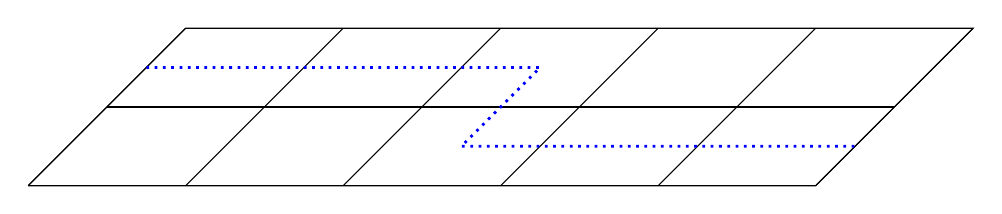
\begin{tikzpicture}[scale=2]
\def\rlvl{0.35}

% Grid
\draw (0,0) -- (1,1) -- (6,1) -- (5,0) -- (0,0);
\foreach \x in {0,1,...,5} {
    \draw (\x,0) -- (\x+1,1);
}
\draw (0.5,0.5) -- (5.5,0.5);

%Path
\draw[line width=0.35mm, blue, dotted] (0.75,0.75) -- (0.75+2.5,0.75) -- (0.75+2.5-0.5,0.75-0.5) -- (0.75+2.5-0.5+2.5,0.75-0.5);

% Raised squares
\raised{(1,0) rectangle (2,\rlvl)}{(2,0) -- (2.5,0.5) -- (2.5,0.5+\rlvl) -- (2,\rlvl)}{(2,\rlvl) -- (2.5,0.5+\rlvl) -- (1.5,0.5+\rlvl) -- (1,\rlvl)}
\raised{(1+2.5,0+0.5) rectangle (2+2.5,\rlvl+0.5)}{(2+2.5,0+0.5) -- (2.5+2.5,0.5+0.5) -- (2.5+2.5,0.5+\rlvl+0.5) -- (2+2.5,\rlvl+0.5)}{(2+2.5,\rlvl+0.5) -- (2.5+2.5,0.5+\rlvl+0.5) -- (1.5+2.5,0.5+\rlvl+0.5) -- (1+2.5,\rlvl+0.5)}
\raised{(1+2.5+1,0+0.5) rectangle (2+2.5+1,\rlvl+0.5)}{(2+2.5+1,0+0.5) -- (2.5+2.5+1,0.5+0.5) -- (2.5+2.5+1,0.5+\rlvl+0.5) -- (2+2.5+1,\rlvl+0.5)}{(2+2.5+1,\rlvl+0.5) -- (2.5+2.5+1,0.5+\rlvl+0.5) -- (1.5+2.5+1,0.5+\rlvl+0.5) -- (1+2.5+1,\rlvl+0.5)}
\end{tikzpicture}
}
    \caption{A grid of length $5$ with three raised squares and a path from left to right.}
    \label{fig:raised_grid}
\end{figure}

Let $G$ be the combinatorial class for passable grids. It is either the empty grid or contains at least one vertical slice. This is described by the admissible constructor disjoint union where a combinatorial class is split into nonintersecting parts. Now we have a combinatorial rule 
\[
    G \cong \set{\varepsilon} \sqcup G_{\geq 1},
\]
where $\varepsilon$ is the empty grid and $G_{\geq 1}$ is the set of passable grid with a positive length. In terms of generating functions this corresponds to addition, that is 
\[
    G(z) = 1 + G_{\geq1}(z).
\] 
Any valid grid consists of a combination of the vertical slices \gridN, \gridU\ and \gridD\ as one with both raised would block the path. We refer to a combinatorial object of length 1 as an \emph{atom}. The generating functions of the empty object and an atom are $1$ and $z$ respectively. Let $A$, $B$ and $C$ be the classes of passable grids starting with \gridN, \gridU\ and \gridD\ respectively and $D$ and $E$ the classes that can follow \gridU\ and \gridD\ respectively. Again we have a disjoint union 
\[
    G_{\geq1} \cong A \sqcup B \sqcup C.
\]
We define $\circ$ as the operator that prepends a vertical slice to all grids in a set. This is a Cartesian product, another admissible constructor denoted by $\times$, where
\[
X \times Y = \cset{(x,y)}{x\in X \text{ and } y \in Y}
\]
and in terms of generating functions corresponds to multiplication. Now we have 
\[
    A \cong \gridN \circ G, \ B \cong \gridU \circ D \text{ and } C \cong \gridD \circ E.
\]
Following \gridU\ can be anything that does not start by blocking the lower square, that is 
\[
    D \cong \set{\varepsilon} \sqcup B \sqcup A
\]
and symmetrically we have 
\[
    E \cong \set{\varepsilon} \sqcup C \sqcup A.
\]
Now we have our specification, a system of rules with each class on the left at most once, defining an unambiguous formal grammar as shown in \FigureRef{fig:gridtree}.

\begin{figure}[ht!]
    \centering
    {
\newcommand{\gridnodeempty}{%
\begin{tikzpicture}[scale=0.3, baseline=(current bounding box.center)]
\useasboundingbox (0,-3) rectangle (3,3);
			\draw[thick, rounded corners=3pt] (0,0) rectangle (3,3);
			\draw[pattern=north west lines, pattern color=lightgray]  (3,0) to[rounded corners=3pt] (0,0) to[rounded corners=3pt] (0,3) to[rounded corners=3pt] (3,3) to[rounded corners=3pt] cycle;
;
			    \end{tikzpicture}
}

\newcommand{\gridnodesingle}[1]{%
\begin{tikzpicture}[scale=0.3, baseline=(current bounding box.center)]
\useasboundingbox (0,-3) rectangle (3,3);
			\draw[thick, rounded corners=3pt] (0,0) rectangle (3,3);
			\node at (1.5, 1.5) {#1};
;
			    \end{tikzpicture}
}


\begin{tikzpicture}[scale=0.8, every node/.style={scale=0.8}]
    \node (root) at (0, 0) {\gridnodesingle{$G$}};
    \node (lvl_1_1) at (-1.5, -2.25) {\gridnodeempty};
    \node (lvl_1_2) at (1.5, -2.25) {\gridnodesingle{$G_{\geq1}$}};
    \node (lvl_2_1) at (-3, -4.5) {\gridnodesingle{$A$}};
    \node (lvl_2_2) at (1.5, -4.5) {\gridnodesingle{$B$}};
    \node (lvl_2_3) at (6, -4.5) {\gridnodesingle{$C$}};
    \node (lvl_3_1) at (-4,-6.75) {\gridnodesingle{\gridN}};
    \node (lvl_3_2) at (-2,-6.75) {\gridnodesingle{$G$}};
    \node (lvl_3_3) at (0.5,-6.75) {\gridnodesingle{$D$}};
    \node (lvl_3_4) at (2.5,-6.75) {\gridnodesingle{\gridU}};
    \node (lvl_3_5) at (5,-6.75) {\gridnodesingle{\gridD}};
    \node (lvl_3_6) at (7,-6.75) {\gridnodesingle{$E$}};
    \node (lvl_4_1) at (-1,-9) {\gridnodeempty};
    \node (lvl_4_2) at (0.5,-9) {\gridnodesingle{$B$}};
    \node (lvl_4_3) at (2,-9) {\gridnodesingle{$A$}};
    \node (lvl_4_4) at (5.5,-9) {\gridnodeempty};
    \node (lvl_4_5) at (7,-9) {\gridnodesingle{$C$}};
    \node (lvl_4_6) at (8.5,-9) {\gridnodesingle{$A$}};
    
    \ptedge{(root)}{(-0.5,1.2)}{(lvl_1_1)}{(-0.5,1.3)}
    \ptedge{(root)}{(-0.5,1.2)}{(lvl_1_2)}{(-0.5,1.3)}
    
    \ptedge{(lvl_1_2)}{(-0.5,1.2)}{(lvl_2_1)}{(-0.5,1.3)}
    \ptedge{(lvl_1_2)}{(-0.5,1.2)}{(lvl_2_2)}{(-0.5,1.3)}
    \ptedge{(lvl_1_2)}{(-0.5,1.2)}{(lvl_2_3)}{(-0.5,1.3)}
    
    \ptedge{(lvl_2_1)}{(-0.5,1.2)}{(lvl_3_1)}{(-0.5,1.3)}
    \ptedge{(lvl_2_1)}{(-0.5,1.2)}{(lvl_3_2)}{(-0.5,1.3)}
    \ptedge{(lvl_2_2)}{(-0.5,1.2)}{(lvl_3_3)}{(-0.5,1.3)}
    \ptedge{(lvl_2_2)}{(-0.5,1.2)}{(lvl_3_4)}{(-0.5,1.3)}
    \ptedge{(lvl_2_3)}{(-0.5,1.2)}{(lvl_3_5)}{(-0.5,1.3)}
    \ptedge{(lvl_2_3)}{(-0.5,1.2)}{(lvl_3_6)}{(-0.5,1.3)}
    
    \ptedge{(lvl_3_3)}{(-0.5,1.2)}{(lvl_4_1)}{(-0.5,1.3)}
    \ptedge{(lvl_3_3)}{(-0.5,1.2)}{(lvl_4_2)}{(-0.5,1.3)}
    \ptedge{(lvl_3_3)}{(-0.5,1.2)}{(lvl_4_3)}{(-0.5,1.3)}
    \ptedge{(lvl_3_6)}{(-0.5,1.2)}{(lvl_4_4)}{(-0.5,1.3)}
    \ptedge{(lvl_3_6)}{(-0.5,1.2)}{(lvl_4_5)}{(-0.5,1.3)}
    \ptedge{(lvl_3_6)}{(-0.5,1.2)}{(lvl_4_6)}{(-0.5,1.3)}
\end{tikzpicture}
}
    \caption{The grammar for passable $2\times n$ grids.}
    \label{fig:gridtree}
\end{figure}

This system of rules when interpreted with generating functions is a set of equations with functions as its unknowns. In our example we have
\[
    \systeme*{G(z) = 1 + G_{\geq1}(z), G_{\geq1}(z) = A(z) + B(z) + C(z),A(z) = zG(z), B(z) = zD(z), C(z) = zE(z), D(z) = 1+B(z)+A(z), E(z) = 1+C(z)+A(z)}
\]
and solving for $G(z)$ gives 
\[
    G(z) = \frac{1+z}{1-2z-z^2}.
\]
The Taylor series for this function, at $z=0$, is
\[
    \sum_{i=0}^\infty \frac{G^{(i)}(0)}{i!}z^i = 1+3z+7z^2+17z^3+ 41z^4 + 99z^5 + \dotsm
\]
which corresponds to the number of grids for each size, e.g., there are 17 and 99 unique passable $2\times3$ and $2\times5$ grids respectively. We can even go further using calculus and find the exact formula, 
\[
|G_n| = \frac{\left(1+\sqrt{2}\right)^{n+1} + \left(1-\sqrt{2}\right)^{n+1}}{2}.
\]
This is not always the case and depends on the type of generating function we have.

In the context of this thesis, we will usually refer to combinatorial classes as just classes and the same goes for combinatorial specifications and rules. We also assume all constructors to be admissible and all rules to entail an isomorphism. 

\section{Permutations\label{sec:permutations}}
A \emph{permutation} $\pi$ is a bijection between a set and itself. In our context, the set in question is $[n] = \setn$. We adopt a one line notation for permutations, $\pi = \perm{\pi}{n}$ where $\pi_i = j$ if $i$ maps to $j$. The permutation $1423$ maps $\{1,2,3,4\}$ to itself. This correspondence can be seen in \FigureRef{fig:perm_example} as well as a geometric representation of the permutation which displays the points $\cset{(i,\pi(i))}{i \in [n]}$ in the Cartesian plane.

\begin{figure}[ht!]
    \centering
    \begin{tikzpicture}[ele/.style={fill=black,circle,minimum width=.8pt,inner sep=1pt},every fit/.style={ellipse,draw,inner sep=15},scale=0.6, every node/.style={scale=0.6}]
    \draw[white] (0,0);
    \node[ele,label=left:$1$] (a1) at (0,4) {};    
    \node[ele,label=left:$2$] (a2) at (0,3) {};    
    \node[ele,label=left:$3$] (a3) at (0,2) {};
    \node[ele,label=left:$4$] (a4) at (0,1) {};
    
    \node[ele,,label=right:$1$] (b1) at (4,4) {};
    \node[ele,,label=right:$2$] (b2) at (4,3) {};
    \node[ele,,label=right:$3$] (b3) at (4,2) {};
    \node[ele,,label=right:$4$] (b4) at (4,1) {};
    
    \node[draw,fit= (a1) (a2) (a3) (a4),minimum width=2cm] {} ;
    \node[draw,fit= (b1) (b2) (b3) (b4),minimum width=2cm] {} ;  
    \draw[->,thick,shorten <=2pt,shorten >=2pt] (a1) -- (b1);
    \draw[->,thick,shorten <=2pt,shorten >=2] (a2) -- (b4);
    \draw[->,thick,shorten <=2pt,shorten >=2] (a3) -- (b2);
    \draw[->,thick,shorten <=2pt,shorten >=2] (a4) -- (b3);
\end{tikzpicture}
\hspace{2cm}
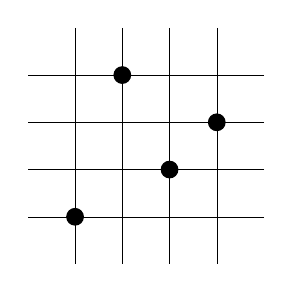
\begin{tikzpicture}[,scale=0.6, every node/.style={scale=0.6}]
        \foreach \x in {1,...,4} {
                \draw[ultra thin] (\x,5)--(\x,0);
                \draw[ultra thin] (5,\x)--(0,\x);
        }
        \draw[fill=black] (1,1) circle (5pt);
        \draw[fill=black] (2,4) circle (5pt);
        \draw[fill=black] (3,2) circle (5pt);
        \draw[fill=black] (4,3) circle (5pt);
\end{tikzpicture}

    \caption{The mapping and graphical representation of the permutation $1423$.}
    \label{fig:perm_example}
\end{figure}

A permutation on $[n]$ is said to be of length $n$ and $\mathcal{S}_n$ is the set of all permutations of length $n$. The set of permutations of length 3 is 
\[
    \mathcal{S}_3 = \{123,132,213,231,312,321\}.
\]
There is a permutation of length $0$, namely the empty permutation, denoted $\varepsilon$. This is the unique map from $\emptyset$ to $\emptyset$. The set of all permutations is denoted by $\mathcal{S}$. It is a combinatorial class since $\mathcal{S}_n$ is finite for all $n\in\N$, containing $n!$ elements.

Given a permutation $\pi = \perm{\pi}{n}$, its \emph{reverse} is
\[
    \rev(\pi) = \pi^\textsf{rev} = \wordrev{\pi}{n}
\]
and its \emph{inverse} is
\[
    \inv(\pi) = \pi^{-1} = \wordidx{\pi}{i}{n}
\]
where $\pi_{i_j} = k$ if $\pi_k = j$. The reverse of $132$ is $231$ and the inverse of $51324$ is $24351$. The reverse and inverse functions generate the dihedral group $D_4$, that is the symmetries of a square using the graphical representation of a permutation. We define these eight symmetry maps as $\sym_1,\sym_2,\dotsc,\sym_8$ as is shown in \TableRef{tab:permsym} which also includes an example for the permutation $1423$.

\begin{table}[ht!]
    \centering
    {
\newcommand{\tsquare}[4]{\adjustbox{valign=t}{\begin{tikzpicture}\fill[white] (-.1,-.1) rectangle (.85,.85);\draw (0,0) rectangle (0.75,0.75); \draw (0,.75) node[xshift=1.4mm,yshift=-1.4mm] {\tiny{$#1$}}; \draw (.75,.75) node[xshift=-1.4mm,yshift=-1.4mm] {\tiny{$#2$}}; \draw (.75,.0) node[xshift=-1.4mm,yshift=1.4mm] {\tiny{$#3$}}; \draw (0,0) node[xshift=1.4mm,yshift=1.4mm] {\tiny{$#4$}};\end{tikzpicture}}}

\newcommand{\sA}{
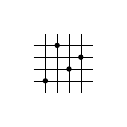
\begin{tikzpicture}[scale=0.15]
    \fill[white] (-.5,-.5) rectangle (5.5,5.5);
    \foreach \x in {1,...,4} {
        \draw[ultra thin] (\x,0)--(\x,5); %vline
        \draw[ultra thin] (0,\x)--(5,\x); %hline
    }
    \draw[fill=black] (1,1) circle (5pt);
    \draw[fill=black] (2,4) circle (5pt);
    \draw[fill=black] (3,2) circle (5pt);
    \draw[fill=black] (4,3) circle (5pt);
\end{tikzpicture}
}

\newcommand{\sB}{
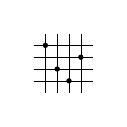
\begin{tikzpicture}[scale=0.15]
    \fill[white] (-.5,-.5) rectangle (5.5,5.5);
    \foreach \x in {1,...,4} {
        \draw[ultra thin] (\x,0)--(\x,5); %vline
        \draw[ultra thin] (0,\x)--(5,\x); %hline
    }
    \draw[fill=black] (1,4) circle (5pt);
    \draw[fill=black] (2,2) circle (5pt);
    \draw[fill=black] (3,1) circle (5pt);
    \draw[fill=black] (4,3) circle (5pt);
\end{tikzpicture}
}

\newcommand{\sC}{
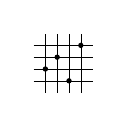
\begin{tikzpicture}[scale=0.15]
    \fill[white] (-.5,-.5) rectangle (5.5,5.5);
    \foreach \x in {1,...,4} {
        \draw[ultra thin] (\x,0)--(\x,5); %vline
        \draw[ultra thin] (0,\x)--(5,\x); %hline
    }
    \draw[fill=black] (1,2) circle (5pt);
    \draw[fill=black] (2,3) circle (5pt);
    \draw[fill=black] (3,1) circle (5pt);
    \draw[fill=black] (4,4) circle (5pt);
\end{tikzpicture}
}

\newcommand{\sD}{
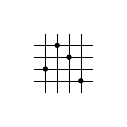
\begin{tikzpicture}[scale=0.15]
    \fill[white] (-.5,-.5) rectangle (5.5,5.5);
    \foreach \x in {1,...,4} {
        \draw[ultra thin] (\x,0)--(\x,5); %vline
        \draw[ultra thin] (0,\x)--(5,\x); %hline
    }
    \draw[fill=black] (1,2) circle (5pt);
    \draw[fill=black] (2,4) circle (5pt);
    \draw[fill=black] (3,3) circle (5pt);
    \draw[fill=black] (4,1) circle (5pt);
\end{tikzpicture}
}

\newcommand{\sE}{
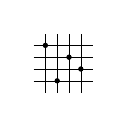
\begin{tikzpicture}[scale=0.15]
    \fill[white] (-.5,-.5) rectangle (5.5,5.5);
    \foreach \x in {1,...,4} {
        \draw[ultra thin] (\x,0)--(\x,5); %vline
        \draw[ultra thin] (0,\x)--(5,\x); %hline
    }
    \draw[fill=black] (1,4) circle (5pt);
    \draw[fill=black] (2,1) circle (5pt);
    \draw[fill=black] (3,3) circle (5pt);
    \draw[fill=black] (4,2) circle (5pt);
\end{tikzpicture}
}

\newcommand{\sF}{
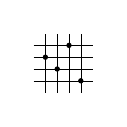
\begin{tikzpicture}[scale=0.15]
    \fill[white] (-.5,-.5) rectangle (5.5,5.5);
    \foreach \x in {1,...,4} {
        \draw[ultra thin] (\x,0)--(\x,5); %vline
        \draw[ultra thin] (0,\x)--(5,\x); %hline
    }
    \draw[fill=black] (1,3) circle (5pt);
    \draw[fill=black] (2,2) circle (5pt);
    \draw[fill=black] (3,4) circle (5pt);
    \draw[fill=black] (4,1) circle (5pt);
\end{tikzpicture}
}

\newcommand{\sG}{
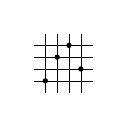
\begin{tikzpicture}[scale=0.15]
    \fill[white] (-.5,-.5) rectangle (5.5,5.5);
    \foreach \x in {1,...,4} {
        \draw[ultra thin] (\x,0)--(\x,5); %vline
        \draw[ultra thin] (0,\x)--(5,\x); %hline
    }
    \draw[fill=black] (1,1) circle (5pt);
    \draw[fill=black] (2,3) circle (5pt);
    \draw[fill=black] (3,4) circle (5pt);
    \draw[fill=black] (4,2) circle (5pt);
\end{tikzpicture}
}

\newcommand{\sH}{
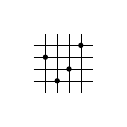
\begin{tikzpicture}[scale=0.15]
    \fill[white] (-.5,-.5) rectangle (5.5,5.5);
    \foreach \x in {1,...,4} {
        \draw[ultra thin] (\x,0)--(\x,5); %vline
        \draw[ultra thin] (0,\x)--(5,\x); %hline
    }
    \draw[fill=black] (1,3) circle (5pt);
    \draw[fill=black] (2,1) circle (5pt);
    \draw[fill=black] (3,2) circle (5pt);
    \draw[fill=black] (4,4) circle (5pt);
\end{tikzpicture}
}

\begin{tabular}{c|c|c|c|c|c}
    \adjustbox{valign=T}{$\textsf{sym}_0$} & \adjustbox{valign=T}{$\pi$} & \adjustbox{valign=T}{Rotate $0^\circ$} & \tsquare{A}{B}{C}{D} & \adjustbox{valign=T}{$1423$} & \adjustbox{valign=t}{\sA} \\
    \hline
    \adjustbox{valign=T}{$\textsf{sym}_1$} & \adjustbox{valign=T}{$\textsf{r}(\textsf{i}(\pi))$} & \adjustbox{valign=T}{Rotate $90^\circ$} & \tsquare{D}{A}{B}{C} & \adjustbox{valign=T}{$4213$} & \adjustbox{valign=t}{\sB}\\
    \hline
    \adjustbox{valign=T}{$\textsf{sym}_2$} & \adjustbox{valign=T}{$\textsf{i}(\textsf{r}(\textsf{i}(\textsf{r}(\pi))))$} & \adjustbox{valign=T}{Rotate $180^\circ$} & \tsquare{C}{D}{A}{B} & \adjustbox{valign=T}{$2314$} &\adjustbox{valign=t}{\sC} \\
    \hline
    \adjustbox{valign=T}{$\textsf{sym}_3$} & \adjustbox{valign=T}{$\textsf{i}(\textsf{r}(\pi))$} & \adjustbox{valign=T}{Rotate $270^\circ$} & \tsquare{B}{C}{D}{A} & \adjustbox{valign=T}{$2431$} & \adjustbox{valign=t}{\sD}\\
    \hline
    \adjustbox{valign=T}{$\textsf{sym}_4$} & \adjustbox{valign=T}{$\textsf{i}(\textsf{r}(\textsf{i}(\pi)))$} & \adjustbox{valign=T}{Horizontal flip} & \tsquare{D}{C}{B}{A} & \adjustbox{valign=T}{$4132$} &\adjustbox{valign=t}{\sE}\\
    \hline
    \adjustbox{valign=T}{$\textsf{sym}_5$} & \adjustbox{valign=T}{$\textsf{r}(\pi)$} & \adjustbox{valign=T}{Vertical flip} & \tsquare{B}{A}{D}{C} & \adjustbox{valign=T}{$3241$} &\adjustbox{valign=t}{\sF}\\
    \hline
    \adjustbox{valign=T}{$\textsf{sym}_6$} & \adjustbox{valign=T}{$\textsf{i}(\pi)$} & \adjustbox{valign=T}{Diagonal flip} & \tsquare{C}{B}{A}{D} & \adjustbox{valign=T}{$1342$} &\adjustbox{valign=t}{\sG}\\
    \hline
    \adjustbox{valign=T}{$\textsf{sym}_7$} & \adjustbox{valign=T}{$\textsf{r}(\textsf{i}(\textsf{r}(\pi)))$} & \adjustbox{valign=T}{Antidiagonal flip} & \tsquare{A}{D}{C}{B} & \adjustbox{valign=T}{$3124$} &\adjustbox{valign=t}{\sH}\\
\end{tabular}

}
    \caption{The eight symmetry maps for permutations interpreted with reverse and inverse, dihedral group $D_4$ and an example for $\pi=1423$.}
    \label{tab:permsym}
\end{table}

We define $\sym(\pi) = \cset{\sym_i(\pi)}{i \in [8]}$ as the \emph{symmetries of} $\pi$. Note that two different symmetry functions can map to the same permutation, e.g., $\sym(1) = \set{1}$. Every permutation has between one and eight symmetries.

Given a finite strictly totally ordered set $(M, <)$ where $M = \set{x_1,x_2,\dotsc,x_n}$, we define its \emph{sorting} as
\[
    \sort(M) = (x_{i_1},x_{i_2},\dotsc,x_{i_n})
\]
if $x_{i_1} < x_{i_2} < \dotsm < x_{i_n}$. Suppose $M=\set{1,5,2}$, then $\sort(M) = (1,2,5)$. The \emph{indexed subsequence} of a permutation $\pi \in \mathcal{S}_n$ for indices $S\subseteq [n]$ is the sequence
\[
    \sseq{S}{\pi}=\wordidx{\pi}{i}{|S|}
\]
if $\sort(S) = (i_1,i_2,\dotsc,i_{|S|})$. Given an indexed subsequence $\gamma$ of a permutation $\pi \in \mathcal{S}_n$, its \emph{standardization}, $\st{\gamma}$, is the sequence where the $i^\text{th}$ largest entry has been replaced by $i$. Let $\pi = 41253 \in \mathcal{S}_5$ and $S=\{1,3,4\}$, then $\st{\sseq{S}{\pi}} = \st{425} = 213$.

Given two permutations $\pi \in \mathcal{S}_n$ and $\sigma \in \mathcal{S}_k$ we say that $\pi$ \emph{contains} $\sigma$, denoted $\contains{\pi}{\sigma}$, if there exists a subset $S \subseteq [n]$ such that $\st{\sseq{S}{\pi}} = \sigma$. If $\pi$ does not contain $\sigma$, it \emph{avoids} it. In the context of containment, we usually refer to the contained permutation as a (\emph{classical}\footnote{There are other types of patterns that we do not concern ourselves with in this thesis.}) \emph{pattern} and that permutations contain or avoid a pattern. The permutation $356214$ contains the pattern $4213$ since
\[
    \st{\sseq{\{2, 4, 5, 6\}}{356214}} = \st{5214} = 4213.
\]
It, however, avoids the pattern $1432$ since
\[
    1432 \notin \cset{\st{\sseq{S}{356214}}}{S \subseteq [6]}.
\]
An occurrence of $4213$ in $356214$ can be seen in \FigureRef{fig:pattern_containment}.

\begin{figure}[ht!]
    \centering
    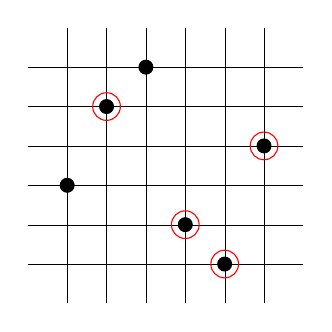
\begin{tikzpicture}[scale=.5,baseline=(current bounding box.center)]
    \foreach \x in {1,...,6} {
        \draw[ultra thin] (\x,0)--(\x,7); %vline
        \draw[ultra thin] (0,\x)--(7,\x); %hline
    }
    \draw[fill=black] (1,3) circle (5pt);
    \draw[fill=black] (2,5) circle (5pt);
    \draw[fill=black] (3,6) circle (5pt);
    \draw[fill=black] (4,2) circle (5pt);
    \draw[fill=black] (5,1) circle (5pt);
    \draw[fill=black] (6,4) circle (5pt);
    \draw[red] (2,5) circle (10pt);
    \draw[red] (4,2) circle (10pt);
    \draw[red] (5,1) circle (10pt);
    \draw[red] (6,4) circle (10pt);
\end{tikzpicture}
    \caption{The permutation $356214$ with an occurrence of $4213$ circled.}
    \label{fig:pattern_containment}
\end{figure}

A set of permutations $\Pi$ is \emph{closed downwards} with respect to containment if 
\[
    \bigcup_{\pi \in \Pi}\cset{\sigma}{\contains{\pi}{\sigma}} \subseteq \Pi.
\]
A set of permutations that is closed downwards is called a \emph{permutation class}. The set $\{\varepsilon, 1, 12, 123\}$ is closed downwards since all patterns contained in any of its elements belong to the set. We can extend this set to include all increasing permutations, $\set{\varepsilon, 1, 12, 123, 1234, \dotsc}$ and it is still closed downwards. Both sets are therefore permutation classes. Isorphism between permutation classes is often called \emph{Wilf equivalence} and their equivalence classes are called \emph{Wilf classes}. 

A permutation $\pi$ \emph{avoids} a set of permutations $\Pi$ if it avoids every $\sigma \in \Pi$. It \emph{contains} $\Pi$ if it does not avoid it, that is, it contains at least one permutation of $\Pi$. Let 
\[
    \Av{\Pi} = \cset{\pi \in \mathcal{S}}{\pi \text{ avoids } \Pi}.
\]
We may abuse this notation by omitting set brackets, writing $\Av{\sigma_1,\sigma_2}$ instead of $\Av{\set{\sigma_1,\sigma_2}}$. Define \[
    \Avn{n}{\Pi} = \cset{\pi \in \Av{\Pi}}{|\pi| = n}
\]
for $n\in\N$.

A set of permutations $\mathcal{B}$ is called a \emph{basis} if for all $\pi\in\mathcal{B}$ there does not exist a $\sigma \in \mathcal{B} \setminus \set{\pi}$ such that $\contains{\pi}{\sigma}$. The set $\{12,21\}$ is a basis while $\{12,231\}$ is not since $\contains{231}{12}$. Permutation classes can be described in terms of a basis avoided, e.g., 
\[
    \{\varepsilon,1,12,123\} = \Av{21, 1234}
\]
and
\[
    \{\varepsilon, 1, 12, 123, 1234,\dotsc\} = \Av{21}.
\]

Let $\mathcal{B}$ be a basis. We extend the definition of symmetry maps to bases such that
\[
    \sym_i(\mathcal{B}) = \cset{\sym_i(\sigma)}{\sigma \in \mathcal{B}}
\]
and
\[
    \sym(\mathcal{B}) = \cset{\sym_i(\mathcal{B})}{i \in [8]}.
\]
For any basis $\mathcal{B}$, the \emph{symmetry class} of $\Av{\mathcal{B}}$ is $\cset{\Av{B}}{B \in \sym(\mathcal{B})}$. The symmetry class of any permutation class is a subset of its Wilf class. As symmetries are considered trivial bijections we usually only concern ourselves with the lexicographically minimal representation of each symmetry class. For example, there are seven symmetry classes and three Wilf classes for singleton bases in $\mathcal{S}_4$. They are shown in \TableRef{tab:wilfcls4}.

\begin{table}[ht!]
    \centering
    \begin{tabular}{c|c}
        Wilf class & Counting sequence\\
        \hline
        $\begin{matrix}\Av{1234}\\\Av{1243}\\\Av{1432}\\\Av{2143}\end{matrix}$ & $1, 2, 6, 23, 103, 513, 2761, 15767, \dotsc$ \\
        \hline
        $\begin{matrix}\Av{1324}\end{matrix}$ & $1, 2, 6, 23, 103, 513, 2762, 15793,\dotsc$\\
        \hline
        $\begin{matrix}\Av{1342}\\\Av{2413}\end{matrix}$ & $1, 2, 6, 23, 103, 512, 2740, 15485,\dotsc$
    \end{tabular}
    \caption{The seven lexicographically minimal representations of symmetry classes of permutation classes avoiding a single classical pattern of length $4$. They are grouped into $3$ Wilf classes.}
    \label{tab:wilfcls4}
\end{table}




\section{Gridded permutations\label{sec:griddedpermutations}}
A \emph{cell} $(a,b) \in \N^2$ is the region within $[0,\infty)^2$ defined by $[a, a+1) \times [b, b+1).$ A pair
\[
    (\pi,P) = (\perm{\pi}{n}, ((a_1,b_1),(a_2,b_2),\dotsc,(a_n,b_n)))
\]
where $P$ is an $n$-tuple of cells and $\pi$ is a permutation is called a \emph{gridded permutation} of length $n$ if for all $i,j \in [n]$, $i<j$ implies $a_i \leq a_j$ and $\pi_i < \pi_j$ implies $b_i \leq b_j$. A more detailed definition is given by Albert \cite{albert2012geometric}. We refer to $P$ as the \emph{positions} of the gridded permutation and $\pi$ as the \emph{underlying permutation}. We use a one line notation for gridded permutations 
\[
    \pi = \pi_1^{(a_1,b_1)}\pi_2^{(a_2,b_2)}\dotsb\pi_n^{(a_n,b_n)}
\]
where we can exclude all but the last position of consecutive occurrences of the same position. The gridded permutation $87^{(0,2)}1^{(1,0)}6^{(1,2)}2^{(1,0)}4^{(3,1)}3^{(3,0)}5^{(4,2)}$ can be seen in \FigureRef{fig:gridded_perm}.

\begin{figure}[ht!]
    \centering
    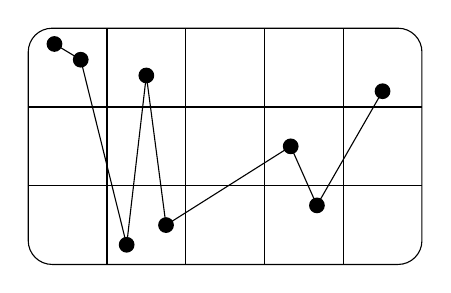
\begin{tikzpicture}
  \def\xs{1.0}
  \def\ys{1.0}
  \def\ps{1.0}
  \draw (0.001,0.001) grid[xscale=\xs,yscale=\ys] (4.999, 2.999);
  \draw[rounded corners=2ex] (0,0) rectangle (5,3);
  \coordinate (p0) at (0.3333333333333333*\xs,2.8*\ys);
  \coordinate (p1) at (0.6666666666666666*\xs,2.6*\ys);
  \coordinate (p2) at (1.25*\xs,0.25*\ys);
  \coordinate (p3) at (1.5*\xs,2.4*\ys);
  \coordinate (p4) at (1.75*\xs,0.5*\ys);
  \coordinate (p5) at (3.3333333333333335*\xs,1.5*\ys);
  \coordinate (p6) at (3.6666666666666665*\xs,0.75*\ys);
  \coordinate (p7) at (4.5*\xs,2.2*\ys);
  \draw (p0)--(p1)--(p2)--(p3)--(p4)--(p5)--(p6)--(p7);
  \fill (p0) circle (0.1*\ps);
  \fill (p1) circle (0.1*\ps);
  \fill (p2) circle (0.1*\ps);
  \fill (p3) circle (0.1*\ps);
  \fill (p4) circle (0.1*\ps);
  \fill (p5) circle (0.1*\ps);
  \fill (p6) circle (0.1*\ps);
  \fill (p7) circle (0.1*\ps);
\end{tikzpicture}
    \caption{The gridded permutation $87^{(0,2)}1^{(1,0)}6^{(1,2)}2^{(1,0)}4^{(3,1)}3^{(3,0)}5^{(4,2)}$.}
    \label{fig:gridded_perm}
\end{figure}

We extend the definition of indexed subsequences to gridded permutations so the sequence produced, $\sseq{S}{\pi}$, contains elements of the underlying permutation and positions. Given this extension, we can also extend the standardization of an indexed subsequence of a gridded permutation to be applied only to the underlying permutation. For example, given a gridded permutation $\pi = 1^{(0,0)}5^{(1,2)}2^{(2,0)}43^{(2,1)}$ and $S=\set{1,2,5}$ we have
\[
\st{\sseq{S}{\pi}} = \st{1^{(0,0)}5^{(1,2)}3^{(2,1)}} = 1^{(0,0)}3^{(1,2)}2^{(2,1)}.
\]
Using the extended definition of standardization we extend containment and avoidance to gridded permutations, for both individual and sets of gridded permutations. For example, the gridded permutation $1^{(0,0)}5^{(1,2)}2^{(2,0)}43^{(2,1)}$ contains $1^{(0,0)}2^{(2,0)}3^{(2,1)}$ but avoids $1^{(0,0)}23^{(2,1)}$.

Let $\mathcal{G}$ be the set of all gridded permutations and $\mathcal{G}_n$ its subset with only gridded permutations of length $n$. The set $\mathcal{G}$ is not a combinatorial class since $\mathcal{G}_n$ is infinite for all $n \in \Z^+$, having infinitely many cells to choose as positions. If we restrict the choice of cells to be finite, then so are the gridded permutations we can form. Let $\mathcal{G}^{(c,r)}$ be the set of gridded permutation with positions in 
\[
\{0,1,\dotsc,c-1\} \times \{0,1,\dotsc,r-1\}
\]
and
\[
\mathcal{G}^{(c,r)}_n = \cset{\pi \in \mathcal{G}^{(c,r)}}{|\pi| = n}.
\]
The set $\mathcal{G}^{(c,r)}$ is a combinatorial class. Define
\[
    \textsf{Av}^{(c,r)}\left(\Pi\right) = \cset{\pi \in \mathcal{G}^{(c,r)}}{\pi \text{ avoids } \Pi}
\]
and
\[
    \textsf{Av}_n^{(c,r)}\left(\Pi\right) = \cset{\pi \in \mathcal{G}_n^{(c,r)}}{\pi \text{ avoids } \Pi}.
\]

\section{Tilings\label{sec:tilings}}
A \emph{tiling} is a triple
\[
\mathcal{T} = ((c,r), \mathcal{O}, \set{\mathcal{R}_1,\mathcal{R}_2,\dotsc,\mathcal{R}_k})
\]
where
\[
    (c,r) \in \Z^+ \times \Z^+, \ \mathcal{O} \subseteq \mathcal{G}^{(c,r)} \text{ and } \mathcal{R}=\set{\mathcal{R}_1,\mathcal{R}_2,\dotsc,\mathcal{R}_k} \subseteq \left(\mathcal{G}^{(c,r)}\right)^k
\]
are called \emph{dimension}, \emph{obstructions} and \emph{requirements} respectively. The gridded permutations in $\textsf{Av}^{(c,r)}\left(\mathcal{O}\right)$ that contain $\mathcal{R}_1,\dotsc,\mathcal{R}_k$ make up the combinatorial class $\textsf{Grid}(\mathcal{T})$. A more detailed definition is given by Bean \cite{BeanPhd:phd}. An example of a tiling can be seen in \FigureRef{fig:tiling_example} where obstructions are red and requirements are blue. Cells with $12$ and $21$ obstruction and a $1$ requirement are represented with a larger black point.

\begin{figure}[ht!]
    \centering
    {
% rect
%\newcommand{\reqpnt}[3]{\fill[blue] (#1-#3,#2-#3) rectangle (#1+#3,#2+#3);}
% donut
%\newcommand{\reqpnt}[3]{\fill[blue] (#1,#2) circle (#3); \fill[white] (#1,#2) circle (#3 * 0.5);}
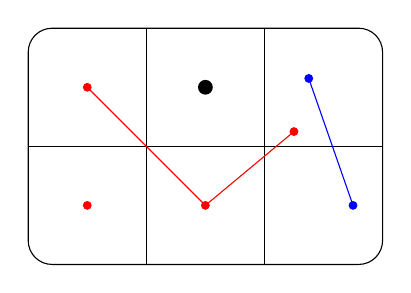
\begin{tikzpicture}[scale=0.75, every node/.style={scale=0.75}]
    \def\spnt{0.075} % Size of smaller points
    \def\lpnt{0.125} % Size of larger points
    \draw[rounded corners=2ex] (0,0) rectangle (6,4);
    \draw (2.0, 4) -- (2.0, 0);
    \draw (4.0, 4) -- (4.0, 0);
    \draw (0, 2) -- (6.0, 2);
    \fill[red] (1, 3) circle (\spnt);
    \fill[red] (1, 1) circle (\spnt);
    \fill[red] (3, 1) circle (\spnt);
    \fill[red] (4.5, 2.25) circle (\spnt);
    \draw[red] (1, 3) -- (3,1) -- (4.5,2.25);
    \fill (3,3) circle (\lpnt);
    \draw[blue] (4.75, 3.15) -- (5.5,1);
    \fill[blue] (4.75, 3.15) circle (\spnt);
    \fill[blue] (5.5, 1) circle (\spnt);
    %\reqpnt{4.75}{3.15}{\spnt*1.2}
    %\reqpnt{5.5}{1}{\spnt*1.2}
\end{tikzpicture}
}
    \caption{A $3 \times 2$ tiling with $\mathcal{R}$ consisting of $\set{1^{(1,1)}}$ and $\set{2^{(1,1)}1^{(2,0)}}$ and $\mathcal{O}$ consisting of $1^{(0,0)}$, $12^{(1,1)}$, $21^{(1,1)}$ and $3^{(0,1)}1^{(1,0)}2^{(2,1)}$.}
    \label{fig:tiling_example}
\end{figure}

Typically, when we want to enumerate $\Av{132}$ we start with a disjoint union constructor since a permutation in $\Av{132}$ is either empty or contains a largest point. If it contains a largest point, it must still avoid 132 on either side. Furthermore, the elements to the left of the largest point must be greater than those to its right or you have an occurrence of $132$ with the largest point. This is important since it allows us to uniquely map the elements to the right of the largest point from the rule. Now we have a specification
\begin{align*}
\Av{132} &\cong \set{\varepsilon} \sqcup \textsf{Av}_{\geq1}(132)\\
\textsf{Av}_{\geq1}(132) &\cong \Av{132} \times \set{\point{0.1}} \times \Av{132}
\end{align*}
and a generating function, obtained by solving the system of equations obtained from the specification,
\[
\frac{1-\sqrt{1-4z}}{2z}.
\]
This is a simple example but given different classes and constructors, we can end up with classes that are difficult to describe accurately. The purpose of tilings is to provide a sort of language to describe classes with more complicated permutation constraints or limited parts of permutations, e.g., we can describe $\textsf{Av}_{\geq1}(132)$ with the tiling seen in \FigureRef{fig:tiling132}.

\begin{figure}[ht!]
    \centering
    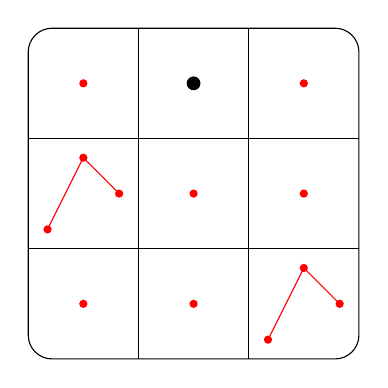
\begin{tikzpicture}[scale=0.7, every node/.style={scale=0.7}]
    \def\spnt{0.075} % Size of smaller points
    \def\lpnt{0.125} % Size of larger points
    \draw[rounded corners=2ex] (0,0) rectangle (6,6);
    \draw (2.0, 6) -- (2.0, 0);
    \draw (4.0, 6) -- (4.0, 0);
    \draw (0, 2) -- (6.0, 2);
    \draw (0, 4) -- (6.0, 4);
    \fill[red] (1, 5) circle (\spnt);
    \fill[red] (1, 1) circle (\spnt);
    \fill[red] (3, 3) circle (\spnt);
    \fill[red] (3, 1) circle (\spnt);
    \fill[red] (5, 5) circle (\spnt);
    \fill[red] (5, 3) circle (\spnt);
    \fill (3,5) circle (\lpnt);
    \draw[red] (0.25+0.1, 2.25+0.1) -- (1,3.75-0.1) -- (1.75-0.1,3);
    \draw[red] (4.25+0.1, 0.25+0.1) -- (5,1.75-0.1) -- (5.75-0.1,1);
    \fill[red] (0.25+0.1, 2.25+0.1) circle (\spnt);
    \fill[red] (1,3.75-0.1) circle (\spnt);
    \fill[red] (1.75-0.1,3) circle (\spnt);
    \fill[red] (4.25+0.1, 0.25+0.1) circle (\spnt);
    \fill[red] (5,1.75-0.1) circle (\spnt);
    \fill[red] (5.75-0.1,1) circle (\spnt);
\end{tikzpicture}
    \caption{A tiling $\mathcal{T}$ with $\textsf{Grid}(\mathcal{T})$ isomorphic to $\textsf{Av}_{\geq1}(132)$.}
    \label{fig:tiling132}
\end{figure}

\section{Combinatorial Exploration}
Combinatorial Exploration \cite{css} is a domain agnostic specification searcher. It uses strategies to generate rules for classes. Strategies are independent of classes and describe an action that may result in rules given an applicable class. The search method is done in a breadth-first manner from the root class. When run, it uses a predefined set of strategies and expands a universe in hope of finding a specification within it.

To avoid tautologies, the searcher gives classes equivalence labels and tracks rules in terms of parent and children pairs as equivalence labels. The rules within a single equivalence label may or may not be equivalence rules. Any single child rule that could result in a tautology could be contained in an equivalence label with nonequivalent classes. When a specification is found and extracted from the universe, any sequence of equivalence rules is merged into a single rule.

\section{TileScope}
TileScope \cite{tiling} is an implementation of Combinatorial Exploration for tilings. The root class usually has a single cell and no requirements and therefore a direct correspondence to a permutation class. The library also utilizes Permuta \cite{permuta}, a general permutation library. Most of the strategies TileScope uses can be found in Bean \cite{BeanPhd:phd}. We will explain those that are not.

\subsection{Column reverse}
\begin{definition}\label{def:rrgp}
Let $\pi=\pi_1^{(x_1,y_1)}\pi_2^{(x_2,y_2)}\dotsm\pi_n^{(x_n,y_n)} \in \mathcal{G}_n$ and define its \emph{column reverse} for $(a,b)\in\N^2$ where $a\leq b$ as the mapping $\textsf{rev}_{[a,b]}$ that reverses the longest subsequence of $\pi$ who's columns all belong to $[a,b]$.
\end{definition}

The column reverse can be extended to tilings such that it is applied to all of its obstructions and requirements. Let $\pi = 5^{(0,1)}2^{(0,0)}4^{(1,1)}1^{(1,0)}6^{(2,2)}3^{(3,1)}$, then $\textsf{rev}_{[1,2]}(\pi) = 5^{(0,1)}2^{(0,0)}6^{(1,2)}1^{(2,0)}4^{(2,1)}3^{(3,1)}$, as shown in \FigureRef{fig:gp_col_rev}. An example for tilings can be seen in \FigureRef{fig:t_col_rev}.

\begin{figure}[ht!]
    \centering
    {
\newcommand{\picw}{1}
\newcommand{\pich}{1}
\begin{tikzpicture}
    \fill[gray!20] (\picw,0) rectangle (3*\picw,3*\pich);
    \draw (1 * \picw, 0) -- (1 * \picw, \pich * 3);
    \draw (2 * \picw, 0) -- (2 * \picw, \pich * 3);
    \draw (3 * \picw, 0) -- (3 * \picw, \pich * 3);
    \draw (0, 1 * \pich) -- (4 * \picw, 1 * \pich);
    \draw (0, 2 * \pich) -- (4 * \picw, 2 * \pich);
    \draw[rounded corners=2ex] (0,0) rectangle (4*\picw,3*\pich);
    \draw (0.25*\picw,3.5*0.5*\pich) -- (0.75*\picw,1*0.5*\pich) -- (1.25*\picw,3*0.5*\pich) -- (1.75*\picw,0.5*0.5*\pich) -- (2.5*\picw,5*0.5*\pich) -- (3.5*\picw,2.5*0.5*\pich);
    \fill (0.25*\picw,3.5*0.5*\pich) circle (0.075) node[below] {$5$};
    \fill (0.75*\picw,1*0.5*\pich) circle (0.075) node[below] {$2$};
    \fill (1.25*\picw,3*0.5*\pich) circle (0.075) node[above] {$4$};
    \fill (1.75*\picw,0.5*0.5*\pich) circle (0.075) node[left] {$1$};
    \fill (2.5*\picw,5*0.5*\pich) circle (0.075) node[above] {$6$};
    \fill (3.5*\picw,2.5*0.5*\pich) circle (0.075) node[above] {$3$};
\end{tikzpicture}
\begin{tikzpicture}
    \draw[white] (0,0) rectangle (2,3*\pich);
    \draw[thick, ->] (0.25,1.5*\pich) -- (1.75,1.5*\pich) node[above,pos=.5] {$\textsf{rev}_{[1,2]}$};
\end{tikzpicture}
\begin{tikzpicture}
    \fill[gray!20] (\picw,0) rectangle (3*\picw,3*\pich);
    \draw (1 * \picw, 0) -- (1 * \picw, \pich * 3);
    \draw (2 * \picw, 0) -- (2 * \picw, \pich * 3);
    \draw (3 * \picw, 0) -- (3 * \picw, \pich * 3);
    \draw (0, 1 * \pich) -- (4 * \picw, 1 * \pich);
    \draw (0, 2 * \pich) -- (4 * \picw, 2 * \pich);
    \draw[rounded corners=2ex] (0,0) rectangle (4*\picw,3*\pich);
    \draw (0.25*\picw,3.5*0.5*\pich) -- (0.75*\picw,1*0.5*\pich) -- (1.5*\picw,5*0.5*\pich) -- (2.25*\picw,0.5*0.5*\pich) -- (2.75*\picw,3*0.5*\pich) -- (3.5*\picw,2.5*0.5*\pich);
    \fill (0.25*\picw,3.5*0.5*\pich) circle (0.075) node[below] {$5$};
    \fill (0.75*\picw,1*0.5*\pich) circle (0.075) node[below] {$2$};
    \fill (1.5*\picw,5*0.5*\pich) circle (0.075) node[above] {$6$};
    \fill (2.25*\picw,0.5*0.5*\pich) circle (0.075) node[right] {$1$};
    \fill (2.75*\picw,3*0.5*\pich) circle (0.075) node[above] {$4$};
    \fill (3.5*\picw,2.5*0.5*\pich) circle (0.075) node[above] {$3$};
\end{tikzpicture}
}
    \caption{The column reverse of a gridded permutation.}
    \label{fig:gp_col_rev}
\end{figure}

\begin{figure}[ht!]
    \centering
    
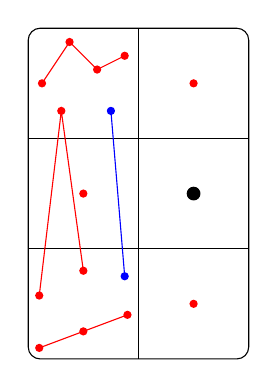
\begin{tikzpicture}[scale=0.7, every node/.style={scale=0.7}]
	\fill (3,3) circle (0.125);
	\fill[red] (1,3) circle (0.075);
	\fill[red] (3,5) circle (0.075);
	\fill[red] (3,1) circle (0.075);
    \draw[rounded corners=1ex] (0,0) rectangle (4,6);
    \draw (0,2) -- (4,2);
    \draw (0,4) -- (4,4);
    \draw (2,0) -- (2,6);
	\coordinate (a1) at (0.2,0.2);
	\coordinate (a2) at (1,0.5);
	\coordinate (a3) at (1.8,0.8);
	\coordinate (b1) at (0.2,1.15);
	\coordinate (b2) at (0.6,4.5);
	\coordinate (b3) at (1,1.6);
	\coordinate (c1) at (0.25,5);
	\coordinate (c2) at (0.75,5.75);
	\coordinate (c3) at (1.25,5.25);
	\coordinate (c4) at (1.75,5.5);
	\coordinate (d1) at (1.5,4.5);
	\coordinate (d2) at (1.75,1.5);
	\fill[red] (a1) circle (0.075);
	\fill[red] (a2) circle (0.075);
	\fill[red] (a3) circle (0.075);
	\fill[red] (b1) circle (0.075);
	\fill[red] (b2) circle (0.075);
	\fill[red] (b3) circle (0.075);
	\fill[red] (c1) circle (0.075);
	\fill[red] (c2) circle (0.075);
	\fill[red] (c3) circle (0.075);
	\fill[red] (c4) circle (0.075);
	\fill[blue] (d1) circle (0.075);
	\fill[blue] (d2) circle (0.075);
	\draw[red] (a1) -- (a2) -- (a3);
	\draw[red] (b1) -- (b2) -- (b3);
	\draw[red] (c1) -- (c2) -- (c3) -- (c4);
	\draw[blue] (d1) -- (d2);
\end{tikzpicture}
\begin{tikzpicture}[scale=0.7]
	\draw[white] (0,0) rectangle (2,6);
	\draw[thick, ->] (-.5,3) -- (2.5,3) node[above,pos=.5] {$\textsf{rev}_{[0,0]}$};
\end{tikzpicture}
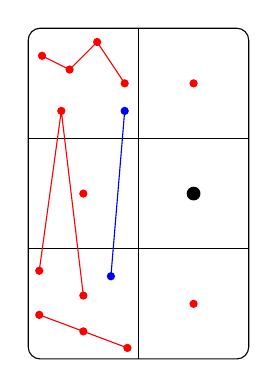
\begin{tikzpicture}[scale=0.7, every node/.style={scale=0.7}]
	\fill (3,3) circle (0.125);
	\fill[red] (1,3) circle (0.075);
	\fill[red] (3,5) circle (0.075);
	\fill[red] (3,1) circle (0.075);
    \draw[rounded corners=1ex] (0,0) rectangle (4,6);
    \draw (0,2) -- (4,2);
    \draw (0,4) -- (4,4);
    \draw (2,0) -- (2,6);
	\coordinate (a1) at (1.8,0.2);
	\coordinate (a2) at (1,0.5);
	\coordinate (a3) at (0.2,0.8);
	\coordinate (b1) at (1,1.15);
	\coordinate (b2) at (0.6,4.5);
	\coordinate (b3) at (0.2,1.6);
	\coordinate (c1) at (1.75,5);
	\coordinate (c2) at (1.25,5.75);
	\coordinate (c3) at (0.75,5.25);
	\coordinate (c4) at (0.25,5.5);
	\coordinate (d1) at (1.75,4.5);
	\coordinate (d2) at (1.5,1.5);
	\fill[red] (a1) circle (0.075);
	\fill[red] (a2) circle (0.075);
	\fill[red] (a3) circle (0.075);
	\fill[red] (b1) circle (0.075);
	\fill[red] (b2) circle (0.075);
	\fill[red] (b3) circle (0.075);
	\fill[red] (c1) circle (0.075);
	\fill[red] (c2) circle (0.075);
	\fill[red] (c3) circle (0.075);
	\fill[red] (c4) circle (0.075);
	\fill[blue] (d1) circle (0.075);
	\fill[blue] (d2) circle (0.075);
	\draw[red] (a1) -- (a2) -- (a3);
	\draw[red] (b1) -- (b2) -- (b3);
	\draw[red] (c1) -- (c2) -- (c3) -- (c4);
	\draw[blue] (d1) -- (d2);
\end{tikzpicture}
    \caption{The column reverse of a tiling.}
    \label{fig:t_col_rev}
\end{figure}

\begin{lemma}\label{lem:crevcontain}
Let $\pi, \sigma \in \mathcal{G}$ such that $\contains{\pi}{\sigma}$, then $\contains{\textsf{rev}_{[a,b]}(\pi)}{\textsf{rev}_{[a,b]}(\sigma)}$.
\end{lemma}
\begin{proof}
If $\pi$ has no elements within the columns then neither does $\sigma$ and both are mapped to themselves. If $\sigma$ has no elements within the columns then the mapping has no effect on the pattern which remains in $\textsf{rev}_{[a,b]}(\pi)$. 

Let $\set{i,i+1,\dotsc,i+k}$ be the indices of elements of $\pi$ within the columns. Let $\sigma = \st{\sseq{A_1\cup L \cup A_2}{\pi}}$ where $L \subseteq \set{i,i+1,\dotsc,i+k}$ and $A_1$ and $A_2$ are the indices in $\pi$ on either side of the columns.

\begin{align*}
    \textsf{rev}_{[a,b]}(\sigma) &= \st{\sseq{A_1}{\pi}\rev\left(\sseq{L}{\pi}\right)\sseq{A_2}{\pi}} \\
    &= \st{\sseq{A_1}{\textsf{rev}_{[a,b]}(\pi)}\sseq{\cset{2i+k-\ell}{\ell \in L}}{\textsf{rev}_{[a,b]}(\pi)}\sseq{A_2}{\textsf{rev}_{[a,b]}(\pi)}}\\
    &= \st{\sseq{A_1 \cup \cset{2i+k-\ell}{\ell \in L} \cup A_2}{\textsf{rev}_{[a,b]}(\pi)}}
\end{align*}
\end{proof}

\begin{lemma}\label{lem:crevgrid}
Let $\mathcal{T}$ be a tiling and $\pi \in \textsf{Grid}(\mathcal{T})$, then $\textsf{rev}_{[a,b]}(\pi)\in\textsf{Grid}(\textsf{rev}_{[a,b]}(\mathcal{T}))$.
\end{lemma}
\begin{proof}
By Lemma \ref{lem:crevcontain} all occurrences of requirements are preserved so the only way that $\textsf{rev}_{[a,b]}(\pi)$ is not in $\textsf{Grid}(\textsf{rev}_{[a,b]}(\mathcal{T}))$ is if there exists an obstruction $o$ that is avoided by $\pi$ while $\textsf{rev}_{[a,b]}(\pi)$ contains $\textsf{rev}_{[a,b]}(o)$. Suppose that there is such an obstruction, then $\textsf{rev}_{[a,b]}(\textsf{rev}_{[a,b]}(\pi)) = \pi$ must contain $\textsf{rev}_{[a,b]}(\textsf{rev}_{[a,b]}(o)) = o$ which contradicts $\pi$ avoiding $o$.
\end{proof}

\begin{proposition}\label{prop:rrtil}
Let $\mathcal{T}$ be a tiling, then $|\textsf{Grid}_n(\mathcal{T})| = |\textsf{Grid}_n(\textsf{rev}_{[a,b]}(\mathcal{T}))|$ for all $n\in\N$.
\end{proposition}
\begin{proof}
For any $\pi \in \textsf{Grid}_n(\mathcal{T})$ we have $(\textsf{rev}_{[a,b]} \circ \textsf{rev}_{[a,b]})(\pi) = \pi$ and therefore $\textsf{rev}_{[a,b]}$ is a bijection between $\textsf{Grid}_n(\mathcal{T})$ and $\cset{\textsf{rev}_{[a,b]}(\pi)}{\pi \in \textsf{Grid}_n(\mathcal{T})}$ with the latter being a subset of $\textsf{Grid}_n(\textsf{rev}_{[a,b]}(\mathcal{T}))$ by Lemma \ref{lem:crevgrid} and therefore $|\textsf{Grid}_n(\mathcal{T})| \leq |\textsf{Grid}_n(\textsf{rev}_{[a,b]}(\mathcal{T}))|$. By the same argument there is a bijection between $\textsf{Grid}_n(\textsf{rev}_{[a,b]}(\mathcal{T}))$ and
\[
    \cset{\textsf{rev}_{[a,b]}(\pi)}{\pi \in \textsf{Grid}_n(\textsf{rev}_{[a,b]}(\mathcal{T}))}
\]
with the latter being a subset of $\textsf{Grid}_n(\textsf{rev}_{[a,b]}(\textsf{rev}_{[a,b]}(\mathcal{T})))=\textsf{Grid}_n(\mathcal{T})$ and therefore $|\textsf{Grid}_b(\mathcal{T})| \geq |\textsf{Grid}(\textsf{rev}_{[a,b]}(\mathcal{T}))|$ and thus $|\textsf{Grid}_n(\mathcal{T})| = |\textsf{Grid}(\textsf{rev}_{[a,b]}(\mathcal{T}))|$
\end{proof}
\subsection{Column permutation}
Let $\pi=\pi_1^{(x_1,y_1)}\pi_2^{(x_2,y_2)}\dotsm\pi_n^{(x_n,y_n)} \in \mathcal{G}_n$ and define $\chi_x(\pi) = \pi_1^{(x,y_1)}\pi_2^{(x,y_2)}\dotsm\pi_n^{(x,y_n)}$, e.g.,
\[
\chi_{1}\left(1^{(0,0)}3^{(2,3)}2^{(5,2)}\right) = 1^{(1,0)}3^{(1,3)}2^{(1,2)}.
\]
This can also be extended to subsequences of gridded permutations.

\begin{definition}
Let $\pi = \pi_1^{(x_1,y_1)}\pi_2^{(x_2,y_2)}\dotsm\pi_n^{(x_n,y_n)} \in \mathcal{G}_n^{(c,r)}$ and $\sigma \in \mathcal{S}_k$ for $k \geq c$. The \emph{column permutation} $\sigma$ of $\pi$ is 
\[
    C_\sigma(\pi) = \chi_0(\sseq{A_{\sigma_1}}{\pi})\chi_1(\sseq{A_{\sigma_2}}{\pi}) \dotsm \chi_{k-1}(\sseq{A_{\sigma_k}}{\pi})
\]
where $A_i = \cset{j \in [n]}{x_j = i - 1}$ for $i \in [k]$.
\end{definition}

Note that $A_1,A_2,\dotsc,A_k$ can include empty sets and $\sigma$ can be larger than the number of columns the gridded permutation spans, but not vice versa. We extend this definition to tilings such that it is applied to all of its obstructions and requirements. Let $\sigma = 4312$ and
\[
\pi = 6^{(0,1)}2^{(0,0)}5^{(1,1)}3^{(1,0)}8^{(1,2)}4^{(2,1)}7^{(3,2)}1^{(3,0)},
\]
then $A_1=\set{1,2}$, $A_2=\set{3,4,5}$, $A_3=\set{6}$, $A_4=\set{7,8}$ and we have
\begin{align*}
    C_\sigma(\pi) &= \chi_0\left(\sseq{A_{\sigma_1}}{\pi}\right)\chi_1\left(\sseq{A_{\sigma_2}}{\pi}\right)\chi_2\left(\sseq{A_{\sigma_3}}{\pi}\right) \chi_3\left(\sseq{A_{\sigma_{4}}}{\pi}\right) \\
    &= \chi_0\left(\sseq{A_{4}}{\pi}\right)\chi_1\left(\sseq{A_{3}}{\pi}\right)\chi_2\left(\sseq{A_{1}}{\pi}\right)\chi_3\left(\sseq{A_{2}}{\pi}\right) \\
    &= \chi_0\left(\sseq{{\set{7,8}}}{\pi}\right) \chi_1\left(\sseq{{\set{6}}}{\pi}\right)\chi_2\left(\sseq{{\set{1,2}}}{\pi}\right)\chi_3\left(\sseq{\set{3,4,5}}{\pi}\right) \\
    &= \chi_0\left(7^{(3,2)}1^{(3,0)}\right)\chi_1\left(4^{(2,1)}\right)\chi_2\left(6^{(0,1)}2^{(0,0)}\right)\chi_3\left(5^{(1,1)}3^{(1,0)}8^{(1,2)}\right) \\
    &= 7^{(0,2)}1^{(0,0)}4^{(1,1)}6^{(2,1)}2^{(2,0)}5^{(3,1)}3^{(3,0)}8^{(3,2)}
\end{align*}
as is shown in \FigureRef{fig:gp_col_perm}. An example for tilings can be seen in \FigureRef{fig:t_col_perm}.

\begin{figure}[ht!]
    \centering
    {
\newcommand{\myscale}{0.7}
\begin{tikzpicture}[scale=\myscale, every node/.style={scale=\myscale}]
    \draw[rounded corners=2ex] (0,0) rectangle (8,6);
    \foreach \x in {2,4,6} {
        \draw (\x,0) -- (\x,6);
    }
    \foreach \y in {2,4} {
        \draw (0,\y) -- (8, \y);
    }
    \draw (0.5,3.5) -- (1.5,1) -- (2.5,3) -- (3,1.5) -- (3.5,5.5) -- (5,2.5) -- (6.5,4.5) -- (7.5,.5);
    
    \fill (0.5,3.5) circle (0.1) node[above] {$6$};
    \fill (1.5,1) circle (0.1) node[below] {$2$};
    \fill (2.5,3) circle (0.1) node[above] {$5$};
    \fill (3,1.5) circle (0.1) node[below] {$3$};
    \fill (3.5,5.5) circle (0.1) node[above] {$8$};
    \fill (5,2.5) circle (0.1) node[below] {$4$};
    \fill (6.5,4.5) circle (0.1) node[above] {$7$};
    \fill (7.5,.5) circle (0.1) node[below] {$1$};
    \foreach \x in {1,2,3,4} {
        \draw (\x*2-1, 0) node[below] {$\x$};
    }
\end{tikzpicture}
\begin{tikzpicture}[scale=\myscale]
    \draw[white] (0,0) rectangle (2,6);
    \draw[thick, ->] (0,3.4) -- (2,3.4) node[above,pos=.5] {$C_{4312}$};
\end{tikzpicture}
\begin{tikzpicture}[scale=\myscale, every node/.style={scale=\myscale}]
    \draw[rounded corners=2ex] (0,0) rectangle (8,6);
    \foreach \x in {2,4,6} {
        \draw (\x,0) -- (\x,6);
    }
    \foreach \y in {2,4} {
        \draw (0,\y) -- (8, \y);
    }
    \draw (0.5,4.5) -- (1.5,.5) -- (3,2.5) -- (4.5,3.5) -- (5.5,1) -- (6.5,3) -- (7,1.5) -- (7.5,5.5);
    \fill (0.5,4.5) circle (0.1) node[above] {$7$};
    \fill (1.5,.5) circle (0.1) node[below] {$1$};
    \fill (3,2.5) circle (0.1) node[below] {$4$};
    \fill (4.5,3.5) circle (0.1) node[above] {$6$};
    \fill (5.5,1) circle (0.1) node[below] {$2$};
    \fill (6.5,3) circle (0.1) node[above] {$5$};
    \fill (7,1.5) circle (0.1) node[below] {$3$};
    \fill (7.5,5.5) circle (0.1) node[above] {$8$};
    \draw (1,0) node[below] {$4$};
    \draw (3,0) node[below] {$3$};
    \draw (5,0) node[below] {$1$};
    \draw (7,0) node[below] {$2$};
\end{tikzpicture}
}
    \caption{The column permutation of a gridded permutation.}
    \label{fig:gp_col_perm}
\end{figure}

\begin{figure}[ht!]
    \centering
    {
\newcommand{\myscale}{0.75}
\begin{tikzpicture}[scale=\myscale, every node/.style={scale=\myscale}]
    \def\xscale{1.0} % Horizontal scale factor
    \def\yscale{0.95} % Vertical scale factor
    \def\spnt{0.075} % Size of smaller points
    \def\lpnt{0.125} % Size of larger points
    \draw[rounded corners=2ex] (0,0) rectangle (6*\xscale,6.26*\yscale);
    \fill[red] (5*\xscale,5.21666665*\yscale) circle (\spnt);
    \fill[red] (5*\xscale,3.13*\yscale) circle (\spnt);
    \fill[red] (3*\xscale,1.04333333*\yscale) circle (\spnt);
    \draw (2.0*\xscale, 6.26*\yscale) -- (2.0*\xscale, 0);
    \draw (4.0*\xscale, 6.26*\yscale) -- (4.0*\xscale, 0);
    \draw (0, 2.0866666666666664*\yscale) -- (6.0*\xscale, 2.0866666666666664*\yscale);
    \draw (0, 4.173333333333333*\yscale) -- (6.0*\xscale, 4.173333333333333*\yscale);
    \fill[red] (2.94*\xscale, 3.2*\yscale) circle (\spnt);
    \fill[red] (5.11*\xscale, 1.47*\yscale) circle (\spnt);
    \draw[red] (2.94*\xscale, 3.2*\yscale) -- (5.11*\xscale,1.47*\yscale);
    \fill[red] (4.498157727557963*\xscale, 1.1773727625023829*\yscale) circle (\spnt);
    \fill[red] (5.39*\xscale, 0.48*\yscale) circle (\spnt);
    \draw[red] (4.498157727557963*\xscale, 1.1773727625023829*\yscale) -- (5.39*\xscale,0.48*\yscale);
    \fill[red] (1.05*\xscale, 1.44*\yscale) circle (\spnt);
    \fill[red] (1.57*\xscale, 1.83*\yscale) circle (\spnt);
    \fill[red] (1.8507434638852711*\xscale, 3.256545283652403*\yscale) circle (\spnt);
    \draw[red] (1.05*\xscale, 1.44*\yscale) -- (1.57*\xscale,1.83*\yscale) -- (1.8507434638852711*\xscale,3.256545283652403*\yscale);
    \fill[red] (0.38*\xscale, 1.5*\yscale) circle (\spnt);
    \fill[red] (1.13*\xscale, 2.1866666666666665*\yscale) circle (\spnt);
    \fill[red] (1.36*\xscale, 2.85*\yscale) circle (\spnt);
    \draw[red] (0.38*\xscale, 1.5*\yscale) -- (1.13*\xscale,2.1866666666666665*\yscale) -- (1.36*\xscale,2.85*\yscale);
    \fill[red] (0.47*\xscale, 0.4256190749161856*\yscale) circle (\spnt);
    \fill[red] (0.99*\xscale, 1.08*\yscale) circle (\spnt);
    \fill[red] (1.53*\xscale, 0.74*\yscale) circle (\spnt);
    \draw[red] (0.47*\xscale, 0.4256190749161856*\yscale) -- (0.99*\xscale,1.08*\yscale) -- (1.53*\xscale,0.74*\yscale);
    \fill[red] (0.8*\xscale, 3.87*\yscale) circle (\spnt);
    \fill[red] (1.01*\xscale, 3.2095352654433555*\yscale) circle (\spnt);
    \fill[red] (1.59*\xscale, 3.5300000000000007*\yscale) circle (\spnt);
    \fill[red] (3.02*\xscale, 5.43*\yscale) circle (\spnt);
    \draw[red] (0.8*\xscale, 3.87*\yscale) -- (1.01*\xscale,3.2095352654433555*\yscale) -- (1.59*\xscale,3.5300000000000007*\yscale) -- (3.02*\xscale,5.43*\yscale);
    \fill[blue] (0.15*\xscale, 4.69*\yscale) circle (\spnt);
    \fill[blue] (0.56*\xscale, 1.97*\yscale) circle (\spnt);
    \draw[blue] (0.15*\xscale, 4.69*\yscale) -- (0.56*\xscale,1.97*\yscale);
\end{tikzpicture}
\begin{tikzpicture}
\draw[white] (0,0) rectangle (2,4);
\draw[thick, ->] (0.25,2.3) -- (1.75,2.3) node[above,pos=.5] {$C_{312}$};
\end{tikzpicture}
\begin{tikzpicture}[scale=\myscale, every node/.style={scale=\myscale}]
    \def\xscale{1.0} % Horizontal scale factor
    \def\yscale{0.95} % Vertical scale factor
    \def\spnt{0.075} % Size of smaller points
    \def\lpnt{0.125} % Size of larger points
    \draw[rounded corners=2ex] (0,0) rectangle (6*\xscale,6.26*\yscale);
    \fill[red] (1*\xscale, 5.21666667*\yscale) circle (\spnt);
    \fill[red] (1*\xscale, 3.13*\yscale) circle (\spnt);
    \fill[red] (5*\xscale, 1.04333333*\yscale) circle (\spnt);
    \draw (2.0*\xscale, 6.26*\yscale) -- (2.0*\xscale, 0);
    \draw (4.0*\xscale, 6.26*\yscale) -- (4.0*\xscale, 0);
    \draw (0, 2.0866666666666664*\yscale) -- (6.0*\xscale, 2.0866666666666664*\yscale);
    \draw (0, 4.173333333333333*\yscale) -- (6.0*\xscale, 4.173333333333333*\yscale);
    \fill[red] (1.71*\xscale, 0.21*\yscale) circle (\spnt);
    \fill[red] (5.32*\xscale, 2.93*\yscale) circle (\spnt);
    \draw[red] (1.71*\xscale, 0.21*\yscale) -- (5.32*\xscale,2.93*\yscale);
    \fill[red] (0.5850604532091456*\xscale, 1.4770759947591205*\yscale) circle (\spnt);
    \fill[red] (1.17*\xscale, 0.7*\yscale) circle (\spnt);
    \draw[red] (0.5850604532091456*\xscale, 1.4770759947591205*\yscale) -- (1.17*\xscale,0.7*\yscale);
    \fill[red] (2.28*\xscale, 1.16*\yscale) circle (\spnt);
    \fill[red] (3.13*\xscale, 1.65*\yscale) circle (\spnt);
    \fill[red] (3.63*\xscale, 2.48*\yscale) circle (\spnt);
    \draw[red] (2.28*\xscale, 1.16*\yscale) -- (3.13*\xscale,1.65*\yscale) -- (3.63*\xscale,2.48*\yscale);
    \fill[red] (2.57*\xscale, 1.69*\yscale) circle (\spnt);
    \fill[red] (2.85*\xscale, 2.59*\yscale) circle (\spnt);
    \fill[red] (3.62*\xscale, 3.1*\yscale) circle (\spnt);
    \draw[red] (2.57*\xscale, 1.69*\yscale) -- (2.85*\xscale,2.59*\yscale) -- (3.62*\xscale,3.1*\yscale);
    \fill[red] (3.01*\xscale, 0.26*\yscale) circle (\spnt);
    \fill[red] (3.34*\xscale, 1.07*\yscale) circle (\spnt);
    \fill[red] (3.68*\xscale, 0.73*\yscale) circle (\spnt);
    \draw[red] (3.01*\xscale, 0.26*\yscale) -- (3.34*\xscale,1.07*\yscale) -- (3.68*\xscale,0.73*\yscale);
    \fill[red] (2.56*\xscale, 3.88*\yscale) circle (\spnt);
    \fill[red] (2.91*\xscale, 3.13*\yscale) circle (\spnt);
    \fill[red] (3.48*\xscale, 3.58*\yscale) circle (\spnt);
    \fill[red] (5.11*\xscale, 5.3*\yscale) circle (\spnt);
    \draw[red] (2.56*\xscale, 3.88*\yscale) -- (2.91*\xscale,3.13*\yscale) -- (3.48*\xscale,3.58*\yscale) -- (5.11*\xscale,5.3*\yscale);
    \fill[blue] (2.1*\xscale, 4.91*\yscale) circle (\spnt);
    \fill[blue] (2.48*\xscale, 1.91*\yscale) circle (\spnt);
    \draw[blue] (2.1*\xscale, 4.91*\yscale) -- (2.48*\xscale,1.91*\yscale);
\end{tikzpicture}
}
    \caption{The column permutation of a tiling.}
    \label{fig:t_col_perm}
\end{figure}

Let $\pi=\pi_1\pi_2 \dotsm \pi_n \in\mathcal{S}_n$ and $A = (i_1, i_2,\dotsc,i_k)$ a finite sequence of length $k$ containing elements from $[n-1]$ and define the \emph{adjacent swap} of $\pi$ (relative to $A$) as
\[
\textsf{AdjSwap}_{A}(\pi) = \begin{cases}
\pi_1\pi_2 \dotsm \pi_{i_1-1}\pi_{i_1+1}\pi_{i_1}\pi_{i_1+2}\pi_{i_1+3} \dotsm \pi_n & \mbox{ if } k = 1,\\
\textsf{AdjSwap}_{(i_2,i_3,\dotsc,i_k)}\left(\textsf{AdjSwap}_{(i_1)}(\pi)\right) & \mbox{ otherwise.}
\end{cases}
\]
Let $\pi = 1423$, then $\textsf{AdjSwap}_{(1,2)}(\pi) = \textsf{AdjSwap}_{(2)}(4123) = 4213$.

\begin{lemma}\label{lem:swap}
Let $\pi = 12\dotsm n \in \textsf{Av}_n(21)$ then
\[
    \cset{\textsf{AdjSwap}_A(\pi)}{A \text{ is a finite sequence of elements from } [n-1]} = \mathcal{S}_n
\]
\end{lemma}
It is well known that permutation groups can be generated by adjacent swaps.\todo{Cite something}

\begin{comment}\begin{proof}
Suppose we can generate $\mathcal{S}_{n-1}$ this way from the permutation in $\textsf{Av}_{n-1}(21)$ and let $\pi = \pi_1 \pi_2 \dotsm \pi_n \in \mathcal{S}_n$ with $\pi_j = n$. Let $A = (i_1,i_2,\dotsc,i_k)$ be the sequence of swaps that turns $12\dotsm (n-1)$ into $\pi_1 \pi_2 \dotsm \pi_{j-1}\pi_{j+1}\dotsm \pi_n \in \mathcal{S}_{n-1}$, then
\begin{align*}
    \textsf{AdjSwap}_{(i_1,i_2,\dotsc,i_k, n-1, n-2,\dotsc,j)}(12\dotsm n) = \pi
\end{align*}
and since this holds for a base case, it holds for all lengths $n\in\N$.
\end{proof}\end{comment}

\begin{proposition}
Let $\mathcal{T} = ((n,m),\mathcal{O},\{\mathcal{R}_1,\dotsc,\mathcal{R}_k\})$ be a tiling. For all $\sigma\in\mathcal{S}_n$ and $i\in\mathbb{N}$ we have $|\textsf{Grid}_i(\mathcal{T})| = |\textsf{Grid}_i\left(C_\sigma(\mathcal{T})\right)|$.
\end{proposition}
\begin{proof}
Swapping two adjacent columns $i$ and $i+1$ can be expressed as compositions of bijective mappings, $\textsf{rev}_{[i,i]} \circ \textsf{rev}_{[i+1,i+1]} \circ \textsf{rev}_{[i,i+1]}$ and by Lemma \ref{lem:swap} we can produce any permutation of columns given adjacent swaps.
\end{proof}
\subsection{Sliding}
Sliding is a generalization (to the setting of tilings) of the sliding lemma described in \citeauthor{slide} \cite[Lemma 2.2]{slide}.

\begin{definition}
Let $\pi = \pi_1^{(x_1,0)}\pi_2^{(x_2,0)}\cdots\pi_n^{(x_n,0)} \in \mathcal{G}^{(c,1)}_n$. We define \emph{sliding} as the map $\Upsilon: \mathcal{G}^{(c,1)}_n \to \mathcal{G}^{(c,1)}_n$ defined as follows.
\begin{enumerate}[a)]
    \item If $\pi$ has no elements in $(1,0)$, we move whatever is in $(0,0)$ to $(1,0)$ and we are done.
    \item If $\pi$ has elements in $(1,0)$, we start by shifting all elements in $(2,0), (3,0), \dotsc, (c-1,0)$ one cell to the right and then we do the following until we have depleted the elements of $\pi$ in $(0,0)$:
    \begin{enumerate}[i.]
        \item If the rightmost element in $(0,0)$ is larger than all elements in $(1,0)$, we move the rightmost element of $(1,0)$ to $(2,0)$ as the leftmost element and then we move the rightmost element of $(0,0)$ to $(1,0)$ as the leftmost element.
        \item If the rightmost element in $(0,0)$ has a larger element in $(1,0)$, then we move the rightmost element of $(0,0)$ to the right of the smallest element in $(1,0)$ that is larger than it and that element is moved to be the leftmost element in $(2,0)$.
    \end{enumerate}
    Finally we shift all elements one cell to the left.
\end{enumerate}
\end{definition}

An example for $3594^{(0,0)}62^{(1,0)}718^{(2,0)}$ can be seen in \FigureRef{fig:slide_gp_example}. This mapping is also outlined in Algorithm~\ref{alg:slidealg}\footnote{Every algorithm in this thesis is accompanied by a Python implementation that can be found at the appropriate repository at \texttt{\href{https://github.com/PermutaTriangle}{https://github.com/PermutaTriangle}}.}.

\begin{algorithm}
{
\setphaserulewidth{.7pt}

\begin{algorithmic}[1]
\Statex \textbf{Input}: A gridded permutation $\pi = \pi_1^{(x_1,0)}\pi_2^{(x_2,0)} \cdots \pi_n^{(x_n,0)} \in \mathcal{G}^{(m,1)}_n$.
\Statex \textbf{Output}: A gridded permutation in $\mathcal{G}_n^{(m,1)}$ with $(0,0)$ slid through $(1,0)$.
\Procedure{slide}{$\pi$}
    \If{$\cset{i}{x_i = 1} = \emptyset$}
        \State \Return{$\pi_1^{(x_1+1-\textsf{sign}(x_1),0)}\pi_2^{(x_2+1-\textsf{sign}(x_2),0)} \cdots \pi_n^{(x_n+1-\textsf{sign}(x_n),0)}$}
    \EndIf
    
    \For{$i \gets |\cset{j}{x_j < 2}| + 1, n$}
        \State $x_i \gets x_i + 1$
    \EndFor
    
    \While{$\cset{j}{x_j = 0} \neq \emptyset$}
        \State $i \gets \max\cset{j}{x_j = 0}$
        \State $A \gets \cset{j}{x_j = 1 \text{ and } \pi_j > \pi_i}$
        \State $k \gets |\cset{j}{x_j < 2}|$
        \If{$A = \emptyset$}
            \State $x_k \gets 2$
            \State $x_i \gets 1$
        \Else
            \State $j \gets \max(A)$
            \State $\alpha \gets \pi_i$
            \State $\beta \gets \pi_j$
            \For{$z\gets i, j-1$}
                \State $\pi_{z}^{(x_z,y_z)} \gets \pi_{z+1}^{(x_{z+1},y_{z+1})}$
            \EndFor
            \State $\pi_{j-1} \gets \alpha$
            \For{$z\gets j, k - 1$}
                \State $\pi_{z}^{(x_z,y_z)} \gets \pi_{z+1}^{(x_{z+1},y_{z+1})}$
            \EndFor
            \State $\pi_{k}^{(x_k,y_k)} \gets \beta^{(2,0)}$
        \EndIf
    \EndWhile
    \State \Return{$\pi_1^{(x_1 - 1,0)}\pi_2^{(x_2 - 1,0)}\cdots\pi_n^{(x_n - 1,0)}$}
\EndProcedure
\end{algorithmic}

}
\caption{The sliding algorithm}
\label{alg:slidealg}
\end{algorithm}

\begin{figure}[ht!]
    \centering
    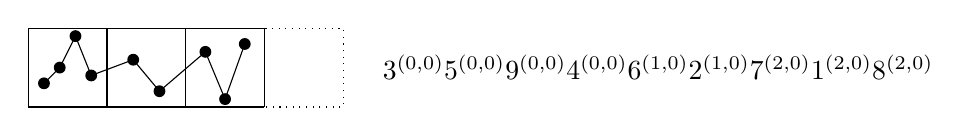
\begin{tikzpicture}
\def\xs{1.0}
\def\ys{1.0}
\def\ps{0.75}
\draw (0,0) grid[xscale=\xs,yscale=\ys] (3, 1);
\draw[dotted] (3*\xs,0) rectangle (4*\xs,1*\xs);
\coordinate (p0) at (0.2*\xs,0.30000000000000004*\ys);
\coordinate (p1) at (0.4*\xs,0.5*\ys);
\coordinate (p2) at (0.6000000000000001*\xs,0.9*\ys);
\coordinate (p3) at (0.8*\xs,0.4*\ys);
\coordinate (p4) at (1.3333333333333333*\xs,0.6000000000000001*\ys);
\coordinate (p5) at (1.6666666666666665*\xs,0.2*\ys);
\coordinate (p6) at (2.25*\xs,0.7000000000000001*\ys);
\coordinate (p7) at (2.5*\xs,0.1*\ys);
\coordinate (p8) at (2.75*\xs,0.8*\ys);
\draw (p0)--(p1)--(p2)--(p3)--(p4)--(p5)--(p6)--(p7)--(p8);
\fill (p0) circle (0.1*\ps);
\fill (p1) circle (0.1*\ps);
\fill (p2) circle (0.1*\ps);
\fill (p3) circle (0.1*\ps);
\fill (p4) circle (0.1*\ps);
\fill (p5) circle (0.1*\ps);
\fill (p6) circle (0.1*\ps);
\fill (p7) circle (0.1*\ps);
\fill (p8) circle (0.1*\ps);
\draw (8,0.5) node {$3^{(0,0)}5^{(0,0)}9^{(0,0)}4^{(0,0)}6^{(1,0)}2^{(1,0)}7^{(2,0)}1^{(2,0)}8^{(2,0)}$};
\end{tikzpicture}

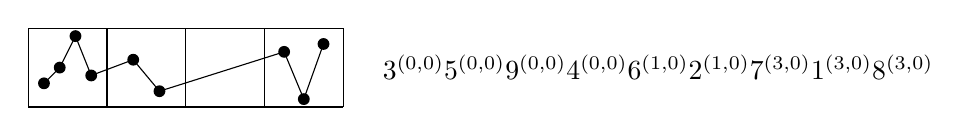
\begin{tikzpicture}
\def\xs{1.0}
\def\ys{1.0}
\def\ps{0.75}
\draw (0,0) grid[xscale=\xs,yscale=\ys] (4, 1);
\coordinate (p0) at (0.2*\xs,0.30000000000000004*\ys);
\coordinate (p1) at (0.4*\xs,0.5*\ys);
\coordinate (p2) at (0.6000000000000001*\xs,0.9*\ys);
\coordinate (p3) at (0.8*\xs,0.4*\ys);
\coordinate (p4) at (1.3333333333333333*\xs,0.6000000000000001*\ys);
\coordinate (p5) at (1.6666666666666665*\xs,0.2*\ys);
\coordinate (p6) at (1+2.25*\xs,0.7000000000000001*\ys);
\coordinate (p7) at (1+2.5*\xs,0.1*\ys);
\coordinate (p8) at (1+2.75*\xs,0.8*\ys);
\draw (p0)--(p1)--(p2)--(p3)--(p4)--(p5)--(p6)--(p7)--(p8);
\fill (p0) circle (0.1*\ps);
\fill (p1) circle (0.1*\ps);
\fill (p2) circle (0.1*\ps);
\fill (p3) circle (0.1*\ps);
\fill (p4) circle (0.1*\ps);
\fill (p5) circle (0.1*\ps);
\fill (p6) circle (0.1*\ps);
\fill (p7) circle (0.1*\ps);
\fill (p8) circle (0.1*\ps);
\draw (8,0.5) node {$3^{(0,0)}5^{(0,0)}9^{(0,0)}4^{(0,0)}6^{(1,0)}2^{(1,0)}7^{(3,0)}1^{(3,0)}8^{(3,0)}$};
\end{tikzpicture}

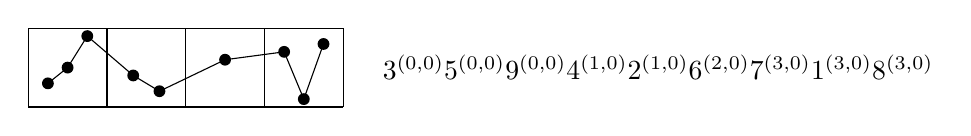
\begin{tikzpicture}
\def\xs{1.0}
\def\ys{1.0}
\def\ps{0.75}
\draw (0,0) grid[xscale=\xs,yscale=\ys] (4, 1);
\coordinate (p0) at (0.25*\xs,0.30000000000000004*\ys);
\coordinate (p1) at (0.5*\xs,0.5*\ys);
\coordinate (p2) at (0.75*\xs,0.9*\ys);
\coordinate (p3) at (1.3333333333333333*\xs,0.4*\ys);
\coordinate (p4) at (1.6666666666666665*\xs,0.2*\ys);
\coordinate (p5) at (2.5*\xs,0.6000000000000001*\ys);
\coordinate (p6) at (3.25*\xs,0.7000000000000001*\ys);
\coordinate (p7) at (3.5*\xs,0.1*\ys);
\coordinate (p8) at (3.75*\xs,0.8*\ys);
\draw (p0)--(p1)--(p2)--(p3)--(p4)--(p5)--(p6)--(p7)--(p8);
\fill (p0) circle (0.1*\ps);
\fill (p1) circle (0.1*\ps);
\fill (p2) circle (0.1*\ps);
\fill (p3) circle (0.1*\ps);
\fill (p4) circle (0.1*\ps);
\fill (p5) circle (0.1*\ps);
\fill (p6) circle (0.1*\ps);
\fill (p7) circle (0.1*\ps);
\fill (p8) circle (0.1*\ps);
\draw (8,0.5) node {$3^{(0,0)}5^{(0,0)}9^{(0,0)}4^{(1,0)}2^{(1,0)}6^{(2,0)}7^{(3,0)}1^{(3,0)}8^{(3,0)}$};
\end{tikzpicture}

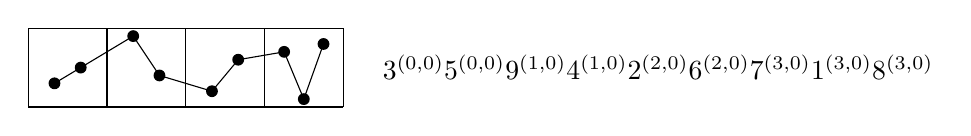
\begin{tikzpicture}
\def\xs{1.0}
\def\ys{1.0}
\def\ps{0.75}
\draw (0,0) grid[xscale=\xs,yscale=\ys] (4, 1);
\coordinate (p0) at (0.3333333333333333*\xs,0.30000000000000004*\ys);
\coordinate (p1) at (0.6666666666666666*\xs,0.5*\ys);
\coordinate (p2) at (1.3333333333333333*\xs,0.9*\ys);
\coordinate (p3) at (1.6666666666666665*\xs,0.4*\ys);
\coordinate (p4) at (2.3333333333333335*\xs,0.2*\ys);
\coordinate (p5) at (2.6666666666666665*\xs,0.6000000000000001*\ys);
\coordinate (p6) at (3.25*\xs,0.7000000000000001*\ys);
\coordinate (p7) at (3.5*\xs,0.1*\ys);
\coordinate (p8) at (3.75*\xs,0.8*\ys);
\draw (p0)--(p1)--(p2)--(p3)--(p4)--(p5)--(p6)--(p7)--(p8);
\fill (p0) circle (0.1*\ps);
\fill (p1) circle (0.1*\ps);
\fill (p2) circle (0.1*\ps);
\fill (p3) circle (0.1*\ps);
\fill (p4) circle (0.1*\ps);
\fill (p5) circle (0.1*\ps);
\fill (p6) circle (0.1*\ps);
\fill (p7) circle (0.1*\ps);
\fill (p8) circle (0.1*\ps);
\draw (8,0.5) node {$3^{(0,0)}5^{(0,0)}9^{(1,0)}4^{(1,0)}2^{(2,0)}6^{(2,0)}7^{(3,0)}1^{(3,0)}8^{(3,0)}$};
\end{tikzpicture}

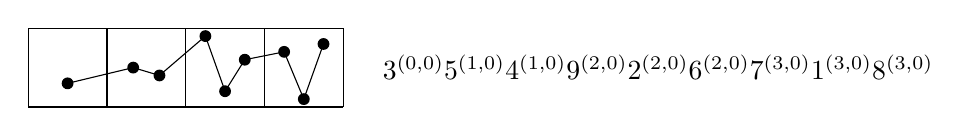
\begin{tikzpicture}
\def\xs{1.0}
\def\ys{1.0}
\def\ps{0.75}
\draw (0,0) grid[xscale=\xs,yscale=\ys] (4, 1);
\coordinate (p0) at (0.5*\xs,0.30000000000000004*\ys);
\coordinate (p1) at (1.3333333333333333*\xs,0.5*\ys);
\coordinate (p2) at (1.6666666666666665*\xs,0.4*\ys);
\coordinate (p3) at (2.25*\xs,0.9*\ys);
\coordinate (p4) at (2.5*\xs,0.2*\ys);
\coordinate (p5) at (2.75*\xs,0.6000000000000001*\ys);
\coordinate (p6) at (3.25*\xs,0.7000000000000001*\ys);
\coordinate (p7) at (3.5*\xs,0.1*\ys);
\coordinate (p8) at (3.75*\xs,0.8*\ys);
\draw (p0)--(p1)--(p2)--(p3)--(p4)--(p5)--(p6)--(p7)--(p8);
\fill (p0) circle (0.1*\ps);
\fill (p1) circle (0.1*\ps);
\fill (p2) circle (0.1*\ps);
\fill (p3) circle (0.1*\ps);
\fill (p4) circle (0.1*\ps);
\fill (p5) circle (0.1*\ps);
\fill (p6) circle (0.1*\ps);
\fill (p7) circle (0.1*\ps);
\fill (p8) circle (0.1*\ps);
\draw (8,0.5) node {$3^{(0,0)}5^{(1,0)}4^{(1,0)}9^{(2,0)}2^{(2,0)}6^{(2,0)}7^{(3,0)}1^{(3,0)}8^{(3,0)}$};
\end{tikzpicture}

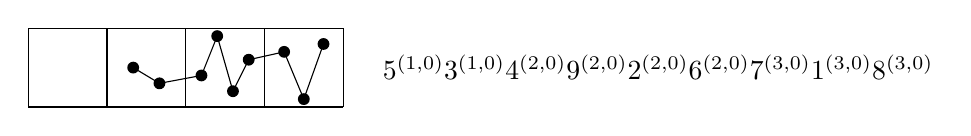
\begin{tikzpicture}
\def\xs{1.0}
\def\ys{1.0}
\def\ps{0.75}
\draw (0,0) grid[xscale=\xs,yscale=\ys] (4, 1);
\coordinate (p0) at (1.3333333333333333*\xs,0.5*\ys);
\coordinate (p1) at (1.6666666666666665*\xs,0.30000000000000004*\ys);
\coordinate (p2) at (2.2*\xs,0.4*\ys);
\coordinate (p3) at (2.4*\xs,0.9*\ys);
\coordinate (p4) at (2.6*\xs,0.2*\ys);
\coordinate (p5) at (2.8*\xs,0.6000000000000001*\ys);
\coordinate (p6) at (3.25*\xs,0.7000000000000001*\ys);
\coordinate (p7) at (3.5*\xs,0.1*\ys);
\coordinate (p8) at (3.75*\xs,0.8*\ys);
\draw (p0)--(p1)--(p2)--(p3)--(p4)--(p5)--(p6)--(p7)--(p8);
\fill (p0) circle (0.1*\ps);
\fill (p1) circle (0.1*\ps);
\fill (p2) circle (0.1*\ps);
\fill (p3) circle (0.1*\ps);
\fill (p4) circle (0.1*\ps);
\fill (p5) circle (0.1*\ps);
\fill (p6) circle (0.1*\ps);
\fill (p7) circle (0.1*\ps);
\fill (p8) circle (0.1*\ps);
\draw (8,0.5) node {$5^{(1,0)}3^{(1,0)}4^{(2,0)}9^{(2,0)}2^{(2,0)}6^{(2,0)}7^{(3,0)}1^{(3,0)}8^{(3,0)}$};
\end{tikzpicture}

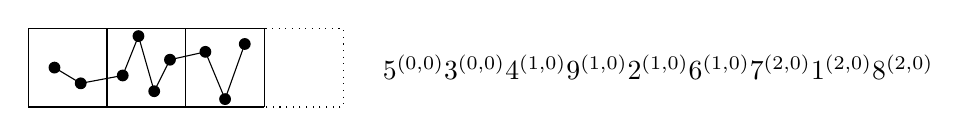
\begin{tikzpicture}
\def\xs{1.0}
\def\ys{1.0}
\def\ps{0.75}
\draw (0,0) grid[xscale=\xs,yscale=\ys] (3, 1);
\draw[dotted] (3*\xs,0) rectangle (4*\xs,1*\xs);
\coordinate (p0) at (-1+1.3333333333333333*\xs,0.5*\ys);
\coordinate (p1) at (-1+1.6666666666666665*\xs,0.30000000000000004*\ys);
\coordinate (p2) at (-1+2.2*\xs,0.4*\ys);
\coordinate (p3) at (-1+2.4*\xs,0.9*\ys);
\coordinate (p4) at (-1+2.6*\xs,0.2*\ys);
\coordinate (p5) at (-1+2.8*\xs,0.6000000000000001*\ys);
\coordinate (p6) at (-1+3.25*\xs,0.7000000000000001*\ys);
\coordinate (p7) at (-1+3.5*\xs,0.1*\ys);
\coordinate (p8) at (-1+3.75*\xs,0.8*\ys);
\draw (p0)--(p1)--(p2)--(p3)--(p4)--(p5)--(p6)--(p7)--(p8);
\fill (p0) circle (0.1*\ps);
\fill (p1) circle (0.1*\ps);
\fill (p2) circle (0.1*\ps);
\fill (p3) circle (0.1*\ps);
\fill (p4) circle (0.1*\ps);
\fill (p5) circle (0.1*\ps);
\fill (p6) circle (0.1*\ps);
\fill (p7) circle (0.1*\ps);
\fill (p8) circle (0.1*\ps);
\draw (8,0.5) node {$5^{(0,0)}3^{(0,0)}4^{(1,0)}9^{(1,0)}2^{(1,0)}6^{(1,0)}7^{(2,0)}1^{(2,0)}8^{(2,0)}$};
\end{tikzpicture}

\begin{tikzpicture}\end{tikzpicture}
    \caption{The sliding of $3594^{(0,0)}62^{(1,0)}718^{(2,0)}$.}
    \label{fig:slide_gp_example}
\end{figure}

\begin{definition}\label{def:slidable}
A pair of tilings
\[
    (\mathcal{T}_1,\mathcal{T}_2) = \left(\left((c,1), \mathcal{O}_1, \set{\mathcal{R}_1,\ldots,\mathcal{R}_k}\right), \left((c,1), \mathcal{O}_2, \set{\mathcal{R}'_1,\ldots,\mathcal{R}'_k}\right)\right)
\]
is \emph{slidable} if the following conditions are satisfied.
\begin{itemize}
    \item The tilings share requirements, that is $\set{\mathcal{R}_1,\ldots,\mathcal{R}_k}=\set{\mathcal{R}'_1,\ldots,\mathcal{R}'_k}$.
    \item No gridded permutation in $\mathcal{R}_1 \cup \cdots \cup \mathcal{R}_k$ has positions in columns $0$ and $1$.
    \item There exists an $n>1$ such that the obstructions $12\cdots n^{(0,0)}, 12\cdots (n-1)^{(0,0)}n^{(1,0)}$ and $12^{(1,0)}$ belong to $\mathcal{O}_1$, $12\cdots n^{(1,0)}, 1^{(0,0)}23\cdots n^{(1,0)}$ and $12^{(0,0)}$ belong to $\mathcal{O}_2$ and no other obstructions that are entirely within columns $0$ and $1$ belong to either $\mathcal{O}_1$ or $\mathcal{O}_2$.
    \item For any obstruction $\pi = \pi_1^{(x_1,0)}\pi_2^{(x_2,0)}\cdots\pi_n^{(x_w,0)} \in \mathcal{O}_1$ with at least one element outside columns $0$ and $1$ the subsequence $\sseq{\cset{i \in [w]}{x_i \in \set{0,1}}}{\pi}$ is either empty or in 
    \[
         \cset{j(j+1)^{(0,0)}, j^{(0,0)}(j+1)^{(1,0)}, j^{(0,0)},j^{(1,0)}}{j\in\Z^+}.
    \]
    Similarly, for $\mathcal{O}_2$, the subsequence must be either empty or in 
    \[
         \cset{j(j+1)^{(1,0)}, j^{(0,0)}(j+1)^{(1,0)}, j^{(0,0)},j^{(1,0)}}{j\in\Z^+}.
    \]
    \item Any obstruction entirely outside columns $0$ and $1$ in $\mathcal{O}_1$ must also exist in $\mathcal{O}_2$ and vice versa.
    \item Let $o_1 = \pi_1^{(0,0)}\pi_2^{(x_2,0)}\cdots\pi_s^{(x_s,0)}$ and $o_2 = \pi_1^{(1,0)}\pi_2^{(x_2,0)}\cdots\pi_s^{(x_s,0)}$ where $x_2,s > 1$ then $o_1 \in \mathcal{O}_1$, $o_2 \in \mathcal{O}_1$, $o_1 \in \mathcal{O}_2$ and $o_2 \in \mathcal{O}_2$ are equivalent. That is, any crossing obstruction with one point in the first two columns must exist in both tilings and with that point in both columns.
    \item Let \begin{align*}o_1 &= \pi_1^{(0,0)}\pi_2^{(0,0)}\pi_3^{(x_3,0)}\cdots\pi_s^{(x_s,0)}\\o_2 &= \pi_1^{(0,0)}\pi_2^{(1,0)}\pi_3^{(x_3,0)}\cdots\pi_s^{(x_s,0)}\\o_3 &= \pi_1^{(1,0)}\pi_2^{(1,0)}\pi_3^{(x_3,0)}\cdots\pi_s^{(x_s,0)}\end{align*} where $s > 2$, $x_3 > 1$ and $\pi_1 + 1 = \pi_2$, then $o_1 \in \mathcal{O}_1$, $o_2 \in \mathcal{O}_1$, $o_2 \in \mathcal{O}_2$ and $o_3 \in \mathcal{O}_2$ are equivalent. That is, any crossing obstruction with $j(j+1)$ in the first two columns (and at least one point outside of those columns) must exists in both tilings where $j(j+1)$ has been spread between the first two columns in all possible ways, excluding the one that collides with the $12$ obstruction.
\end{itemize}
\end{definition}

An example of two slidable tilings can be seen in \FigureRef{fig:slidable_tilings}.

\begin{figure}[ht]
    \centering
    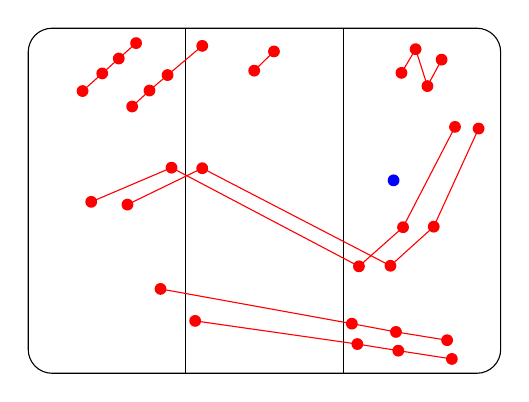
\begin{tikzpicture}[scale=1, every node/.style={scale=1}]
\def\xscale{1.0} % Horizontal scale factor
\def\yscale{0.7} % Vertical scale factor
\def\spnt{0.075} % Size of smaller points
\def\lpnt{0.125} % Size of larger points
\draw[rounded corners=2ex] (0,0) rectangle (6*\xscale,6.26*\yscale);
\draw (2.0*\xscale, 6.26*\yscale) -- (2.0*\xscale, 0);
\draw (4.0*\xscale, 6.26*\yscale) -- (4.0*\xscale, 0);
\fill[red] (2.87*\xscale, 5.49*\yscale) circle (\spnt);
\fill[red] (3.1209520279019056*\xscale, 5.838779282906702*\yscale) circle (\spnt);
\draw[red] (2.87*\xscale, 5.49*\yscale) -- (3.1209520279019056*\xscale,5.838779282906702*\yscale);
\fill[red] (0.69*\xscale, 5.12*\yscale) circle (\spnt);
\fill[red] (0.94*\xscale, 5.44*\yscale) circle (\spnt);
\fill[red] (1.15*\xscale, 5.71*\yscale) circle (\spnt);
\fill[red] (1.37*\xscale, 5.99*\yscale) circle (\spnt);
\draw[red] (0.69*\xscale, 5.12*\yscale) -- (0.94*\xscale,5.44*\yscale) -- (1.15*\xscale,5.71*\yscale) -- (1.37*\xscale,5.99*\yscale);
\fill[red] (1.32*\xscale, 4.84*\yscale) circle (\spnt);
\fill[red] (1.54*\xscale, 5.13*\yscale) circle (\spnt);
\fill[red] (1.77*\xscale, 5.41*\yscale) circle (\spnt);
\fill[red] (2.21*\xscale, 5.94*\yscale) circle (\spnt);
\draw[red] (1.32*\xscale, 4.84*\yscale) -- (1.54*\xscale,5.13*\yscale) -- (1.77*\xscale,5.41*\yscale) -- (2.21*\xscale,5.94*\yscale);
\fill[red] (4.74*\xscale, 5.45*\yscale) circle (\spnt);
\fill[red] (4.92*\xscale, 5.88*\yscale) circle (\spnt);
\fill[red] (5.07*\xscale, 5.21*\yscale) circle (\spnt);
\fill[red] (5.25*\xscale, 5.69*\yscale) circle (\spnt);
\draw[red] (4.74*\xscale, 5.45*\yscale) -- (4.92*\xscale,5.88*\yscale) -- (5.07*\xscale,5.21*\yscale) -- (5.25*\xscale,5.69*\yscale);
\fill[red] (1.68*\xscale, 1.53*\yscale) circle (\spnt);
\fill[red] (4.11*\xscale, 0.9*\yscale) circle (\spnt);
\fill[red] (4.67*\xscale, 0.75*\yscale) circle (\spnt);
\fill[red] (5.32*\xscale, 0.6*\yscale) circle (\spnt);
\draw[red] (1.68*\xscale, 1.53*\yscale) -- (4.11*\xscale,0.9*\yscale) -- (4.67*\xscale,0.75*\yscale) -- (5.32*\xscale,0.6*\yscale);
\fill[red] (2.12*\xscale, 0.95*\yscale) circle (\spnt);
\fill[red] (4.18*\xscale, 0.53*\yscale) circle (\spnt);
\fill[red] (4.7*\xscale, 0.41*\yscale) circle (\spnt);
\fill[red] (5.38*\xscale, 0.26*\yscale) circle (\spnt);
\draw[red] (2.12*\xscale, 0.95*\yscale) -- (4.18*\xscale,0.53*\yscale) -- (4.7*\xscale,0.41*\yscale) -- (5.38*\xscale,0.26*\yscale);
\fill[red] (0.8*\xscale, 3.11*\yscale) circle (\spnt);
\fill[red] (1.82*\xscale, 3.73*\yscale) circle (\spnt);
\fill[red] (4.2*\xscale, 1.94*\yscale) circle (\spnt);
\fill[red] (4.76*\xscale, 2.65*\yscale) circle (\spnt);
\fill[red] (5.42*\xscale, 4.47*\yscale) circle (\spnt);
\draw[red] (0.8*\xscale, 3.11*\yscale) -- (1.82*\xscale,3.73*\yscale) -- (4.2*\xscale,1.94*\yscale) -- (4.76*\xscale,2.65*\yscale) -- (5.42*\xscale,4.47*\yscale);
\fill[red] (1.26*\xscale, 3.06*\yscale) circle (\spnt);
\fill[red] (2.21*\xscale, 3.72*\yscale) circle (\spnt);
\fill[red] (4.6*\xscale, 1.95*\yscale) circle (\spnt);
\fill[red] (5.15*\xscale, 2.66*\yscale) circle (\spnt);
\fill[red] (5.72*\xscale, 4.44*\yscale) circle (\spnt);
\draw[red] (1.26*\xscale, 3.06*\yscale) -- (2.21*\xscale,3.72*\yscale) -- (4.6*\xscale,1.95*\yscale) -- (5.15*\xscale,2.66*\yscale) -- (5.72*\xscale,4.44*\yscale);
\fill[blue] (4.64*\xscale, 3.5*\yscale) circle (\spnt);
\end{tikzpicture}
\hspace{0.5cm}
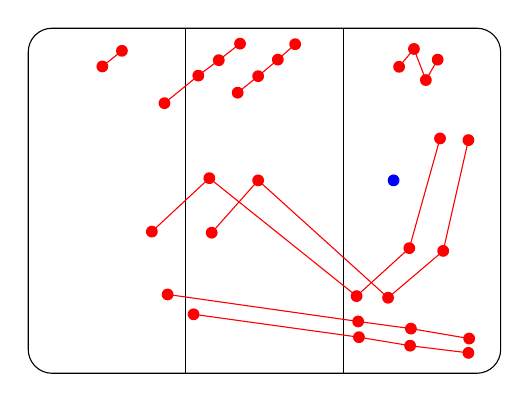
\begin{tikzpicture}[scale=1, every node/.style={scale=1}]
\def\xscale{1.0} % Horizontal scale factor
\def\yscale{0.7} % Vertical scale factor
\def\spnt{0.075} % Size of smaller points
\def\lpnt{0.125} % Size of larger points
\draw[rounded corners=2ex] (0,0) rectangle (6*\xscale,6.26*\yscale);
\draw (2.0*\xscale, 6.26*\yscale) -- (2.0*\xscale, 0);
\draw (4.0*\xscale, 6.26*\yscale) -- (4.0*\xscale, 0);
\fill[red] (0.9413254253242579*\xscale, 5.5665123438541855*\yscale) circle (\spnt);
\fill[red] (1.19*\xscale, 5.85*\yscale) circle (\spnt);
\draw[red] (0.9413254253242579*\xscale, 5.5665123438541855*\yscale) -- (1.19*\xscale,5.85*\yscale);
\fill[red] (1.73*\xscale, 4.9*\yscale) circle (\spnt);
\fill[red] (2.16*\xscale, 5.4*\yscale) circle (\spnt);
\fill[red] (2.42*\xscale, 5.68*\yscale) circle (\spnt);
\fill[red] (2.69*\xscale, 5.98*\yscale) circle (\spnt);
\draw[red] (1.73*\xscale, 4.9*\yscale) -- (2.16*\xscale,5.4*\yscale) -- (2.42*\xscale,5.68*\yscale) -- (2.69*\xscale,5.98*\yscale);
\fill[red] (2.66*\xscale, 5.09*\yscale) circle (\spnt);
\fill[red] (2.92*\xscale, 5.39*\yscale) circle (\spnt);
\fill[red] (3.17*\xscale, 5.69*\yscale) circle (\spnt);
\fill[red] (3.39*\xscale, 5.97*\yscale) circle (\spnt);
\draw[red] (2.66*\xscale, 5.09*\yscale) -- (2.92*\xscale,5.39*\yscale) -- (3.17*\xscale,5.69*\yscale) -- (3.39*\xscale,5.97*\yscale);
\fill[red] (4.71*\xscale, 5.56*\yscale) circle (\spnt);
\fill[red] (4.898395663501238*\xscale, 5.884152285333065*\yscale) circle (\spnt);
\fill[red] (5.05*\xscale, 5.32*\yscale) circle (\spnt);
\fill[red] (5.2*\xscale, 5.69*\yscale) circle (\spnt);
\draw[red] (4.71*\xscale, 5.56*\yscale) -- (4.898395663501238*\xscale,5.884152285333065*\yscale) -- (5.05*\xscale,5.32*\yscale) -- (5.2*\xscale,5.69*\yscale);
\fill[red] (1.77*\xscale, 1.43*\yscale) circle (\spnt);
\fill[red] (4.19*\xscale, 0.94*\yscale) circle (\spnt);
\fill[red] (4.86*\xscale, 0.81*\yscale) circle (\spnt);
\fill[red] (5.6*\xscale, 0.63*\yscale) circle (\spnt);
\draw[red] (1.77*\xscale, 1.43*\yscale) -- (4.19*\xscale,0.94*\yscale) -- (4.86*\xscale,0.81*\yscale) -- (5.6*\xscale,0.63*\yscale);
\fill[red] (2.1*\xscale, 1.07*\yscale) circle (\spnt);
\fill[red] (4.2*\xscale, 0.6546404918137944*\yscale) circle (\spnt);
\fill[red] (4.85*\xscale, 0.5*\yscale) circle (\spnt);
\fill[red] (5.59*\xscale, 0.37*\yscale) circle (\spnt);
\draw[red] (2.1*\xscale, 1.07*\yscale) -- (4.2*\xscale,0.6546404918137944*\yscale) -- (4.85*\xscale,0.5*\yscale) -- (5.59*\xscale,0.37*\yscale);
\fill[red] (1.57*\xscale, 2.57*\yscale) circle (\spnt);
\fill[red] (2.3*\xscale, 3.54*\yscale) circle (\spnt);
\fill[red] (4.17*\xscale, 1.4*\yscale) circle (\spnt);
\fill[red] (4.84*\xscale, 2.27*\yscale) circle (\spnt);
\fill[red] (5.23*\xscale, 4.26*\yscale) circle (\spnt);
\draw[red] (1.57*\xscale, 2.57*\yscale) -- (2.3*\xscale,3.54*\yscale) -- (4.17*\xscale,1.4*\yscale) -- (4.84*\xscale,2.27*\yscale) -- (5.23*\xscale,4.26*\yscale);
\fill[red] (2.33*\xscale, 2.55*\yscale) circle (\spnt);
\fill[red] (2.92*\xscale, 3.5*\yscale) circle (\spnt);
\fill[red] (4.57*\xscale, 1.37*\yscale) circle (\spnt);
\fill[red] (5.27*\xscale, 2.22*\yscale) circle (\spnt);
\fill[red] (5.59*\xscale, 4.23*\yscale) circle (\spnt);
\draw[red] (2.33*\xscale, 2.55*\yscale) -- (2.92*\xscale,3.5*\yscale) -- (4.57*\xscale,1.37*\yscale) -- (5.27*\xscale,2.22*\yscale) -- (5.59*\xscale,4.23*\yscale);
\fill[blue] (4.64*\xscale, 3.5*\yscale) circle (\spnt);
\end{tikzpicture}
    \caption{Typical slidable tilings.}
    \label{fig:slidable_tilings}
\end{figure}

\begin{lemma}\label{lem:slidemap}
Let $(\mathcal{T}_1,\mathcal{T}_2)$ be slidable and $i \in \N$, then $\Upsilon(\pi) \in \textsf{Grid}_i(\mathcal{T}_2)$ for every $\pi \in \textsf{Grid}_i(\mathcal{T}_1)$.
\end{lemma}
\begin{proof}
If $\pi$ contains no elements within the first two columns it is mapped to itself and since the tilings share requirements and are identical outside the first two columns then $\Upsilon(\pi) \in \textsf{Grid}_i(\mathcal{T}_2)$. If $\pi$ contains no elements in column $1$ then whatever is in column $0$ is moved to column $1$. Since $\pi$ avoided $12\dotsm n$ in column $0$ it will also do so in column $1$ once moved and any crossing obstruction in $\mathcal{T}_2$ with one or two points in column $1$ would have existed with those points in column $0$ in $\mathcal{T}_1$ and therefore $\Upsilon(\pi) \in \textsf{Grid}_i(\mathcal{T}_2)$.

Now suppose $\pi$ has elements in column $1$. By the end of the mapping all columns are shifted one to the left but we will refer to their indices before the shift in the mapped tiling. Note that the mapping is defined by placing elements in-order into column $1$ so we will never form an increasing pattern there. 

Suppose after a single step in the map that we form the first $12\cdots n$ (spread in any way across the first $3$ columns). Note that it can contain at most one point in column $1$ as that column is decreasing.

If the $12\cdots n$ pattern does contain the newly moved point in column $1$ and not the one we just moved to column $2$, then the pattern must have been there before the step was taken.

\begin{center}
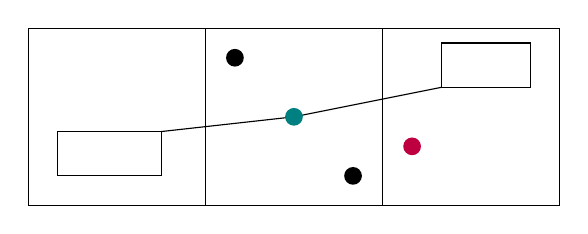
\begin{tikzpicture}[scale=0.75]
    \draw (2.25,1.25) -- (4.5,1.5) -- (7,2);
    \draw (0,0) rectangle (3,3);
    \draw (3,0) rectangle (6,3);
    \draw (6,0) rectangle (9,3);
    \fill (3.5,2.5) circle (0.15);
    \fill[teal] (4.5,1.5) circle (0.15);
    \fill (5.5,0.5) circle (0.15);
    \draw (0.5,0.5) rectangle (2.25,1.25);
    \fill[purple] (6.5,1) circle (0.15);
    \draw (7,2) rectangle (8.5,2.75);
\end{tikzpicture}
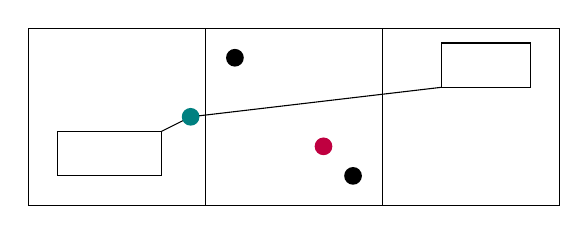
\begin{tikzpicture}[scale=0.75]
    \draw (2.25,1.25) -- (2.75,1.5) -- (7,2);
    \draw (0,0) rectangle (3,3);
    \draw (3,0) rectangle (6,3);
    \draw (6,0) rectangle (9,3);
    \fill (3.5,2.5) circle (0.15);
    \fill[teal] (2.75,1.5) circle (0.15);
    \fill (5.5,0.5) circle (0.15);
    \draw (0.5,0.5) rectangle (2.25,1.25);
    \fill[purple] (5,1) circle (0.15);
    \draw (7,2) rectangle (8.5,2.75);
\end{tikzpicture}
\end{center}

Suppose this pattern includes the newly moved element in column $2$ and no elements in column $1$ then the pattern must have existed before regardless of whether the new element in column $2$ was the smallest element in column $1$ before the move or not.

\begin{center}
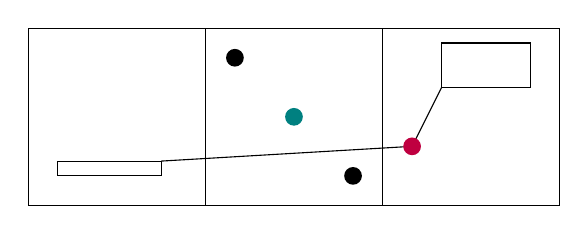
\begin{tikzpicture}[scale=0.75]
    \draw (2.25,0.75) -- (6.5,1) -- (7,2);
    \draw (0,0) rectangle (3,3);
    \draw (3,0) rectangle (6,3);
    \draw (6,0) rectangle (9,3);
    \fill (3.5,2.5) circle (0.15);
    \fill[teal] (4.5,1.5) circle (0.15);
    \fill (5.5,0.5) circle (0.15);
    \draw (0.5,0.5) rectangle (2.25,0.75);
    \fill[purple] (6.5,1) circle (0.15);
    \draw (7,2) rectangle (8.5,2.75);
\end{tikzpicture}
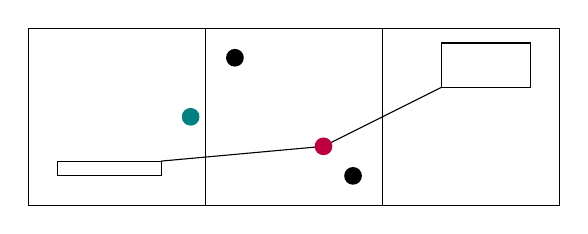
\begin{tikzpicture}[scale=0.75]
    \draw (2.25,0.75) -- (5,1) -- (7,2);
    \draw (0,0) rectangle (3,3);
    \draw (3,0) rectangle (6,3);
    \draw (6,0) rectangle (9,3);
    \fill (3.5,2.5) circle (0.15);
    \fill[teal] (2.75,1.5) circle (0.15);
    \fill (5.5,0.5) circle (0.15);
    \draw (0.5,0.5) rectangle (2.25,0.75);
    \fill[purple] (5,1) circle (0.15);
    \draw (7,2) rectangle (8.5,2.75);
\end{tikzpicture}
\end{center}

Finally suppose the pattern involves elements from both columns $1$ and $2$. Here two scenario can arise. One were the pattern involves both moved elements and the other only the one moved to column $2$. In the first one the pattern remains as we move both points together when we backtrack.

\begin{center}
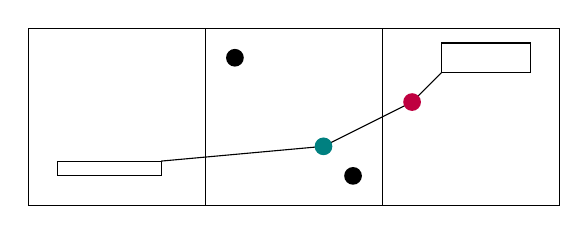
\begin{tikzpicture}[scale=0.75]
    \draw (2.25,0.75) -- (5,1) -- (6.5,1.75) -- (7,2.25);
    \draw (0,0) rectangle (3,3);
    \draw (3,0) rectangle (6,3);
    \draw (6,0) rectangle (9,3);
    \fill (3.5,2.5) circle (0.15);
    \fill[teal] (5,1) circle (0.15);
    \fill (5.5,0.5) circle (0.15);
    \draw (0.5,0.5) rectangle (2.25,0.75);
    \fill[purple] (6.5,1.75) circle (0.15);
    \draw (7,2.25) rectangle (8.5,2.75);
\end{tikzpicture}
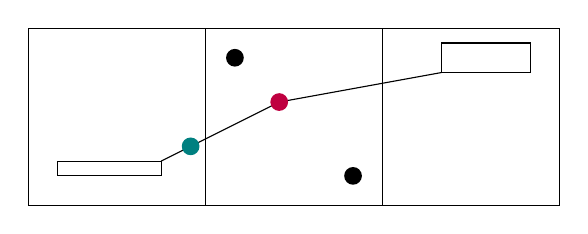
\begin{tikzpicture}[scale=0.75]
    \draw (2.25,0.75) -- (2.75,1) -- (4.25,1.75) -- (7,2.25);
    \draw (0,0) rectangle (3,3);
    \draw (3,0) rectangle (6,3);
    \draw (6,0) rectangle (9,3);
    \fill (3.5,2.5) circle (0.15);
    \fill[teal] (2.75,1) circle (0.15);
    \fill (5.5,0.5) circle (0.15);
    \draw (0.5,0.5) rectangle (2.25,0.75);
    \fill[purple] (4.25,1.75) circle (0.15);
    \draw (7,2.25) rectangle (8.5,2.75);
\end{tikzpicture}
\end{center}

In the latter, there is a smaller element in column $1$ than the moved one that belongs to the pattern. When we go back, the moved element goes back from column $1$ to column $0$ but that is between the element in column $1$ that formed the pattern and the element that was moved to column $2$, preserving the pattern.

\begin{center}
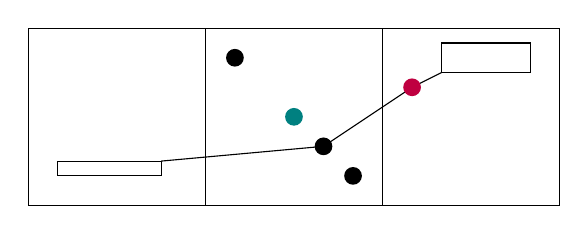
\begin{tikzpicture}[scale=0.75]
    \draw (2.25,0.75) -- (5,1) -- (6.5,2) -- (7,2.25);
    \draw (0,0) rectangle (3,3);
    \draw (3,0) rectangle (6,3);
    \draw (6,0) rectangle (9,3);
    \fill (5.5,0.5) circle (0.15);
    \fill (5,1) circle (0.15);
    \fill[teal] (4.5,1.5) circle (0.15);
    \fill[purple] (6.5,2) circle (0.15);
    \fill (3.5,2.5) circle (0.15);
    \draw (0.5,0.5) rectangle (2.25,0.75);
    \draw (7,2.25) rectangle (8.5,2.75);
\end{tikzpicture}
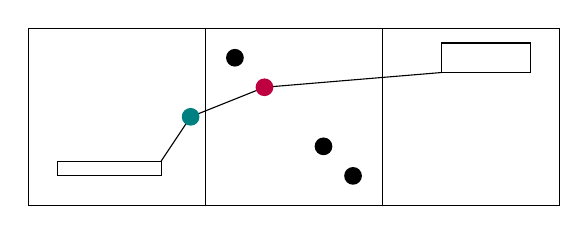
\begin{tikzpicture}[scale=0.75]
    \draw (2.25,0.75) -- (2.75,1.5) -- (4,2) -- (7,2.25);
    \draw (0,0) rectangle (3,3);
    \draw (3,0) rectangle (6,3);
    \draw (6,0) rectangle (9,3);
    \fill (5.5,0.5) circle (0.15);
    \fill (5,1) circle (0.15);
    \fill[teal] (2.75,1.5) circle (0.15);
    \fill[purple] (4,2) circle (0.15);
    \fill (3.5,2.5) circle (0.15);
    \draw (0.5,0.5) rectangle (2.25,0.75);
    \draw (7,2.25) rectangle (8.5,2.75);
\end{tikzpicture}
\end{center}

In the case of the first crossing obstructions forming for the first time with one element in the first 3 columns and some outside, then wherever that element was before must have been an occurrence of that pattern as well.

Now suppose we form the crossing pattern with the elements $k(k+1)$ in the first three columns (spread in any way) for the first time. This can happen in several ways. Note that the two increasing elements can not both be in column $1$ as it is always decreasing.

Suppose the $k(k+1)$ part in the first $3$ columns occurs between the first two, then the pattern must have existed before with $k(k+1)$ in column $0$.

\begin{center}
\begin{tikzpicture}[scale=0.63]
    \coordinate (a1) at (5.5,0.5);
    \coordinate (a2) at (2.75,1);
    \coordinate (a3) at (4.5,1.5);
    \coordinate (a4) at (6.25,2);
    \coordinate (a5) at (3.5,2.5);
    \draw (a2) -- (a3) -- (9.25,1.5);
    \draw (0,0) rectangle (3,3);
    \draw (3,0) rectangle (6,3);
    \draw (6,0) rectangle (9,3);
    \draw (9,0) rectangle (12,3);
    \fill (a1) circle (0.15);
    \fill (a2) circle (0.15);
    \fill[teal] (a3) circle (0.15);
    \fill[purple] (a4) circle (0.15);
    \fill (a5) circle (0.15);
    \draw (9.25,0.25) rectangle (11.75,2.75);
\end{tikzpicture}
\begin{tikzpicture}[scale=0.63]
    \coordinate (a1) at (5.5,0.5);
    \coordinate (a2) at (2.25,1);
    \coordinate (a3) at (2.75,1.5);
    \coordinate (a4) at (4,2);
    \coordinate (a5) at (3.5,2.5);
    \draw (a2) -- (a3) -- (9.25,1.5);
    \draw (0,0) rectangle (3,3);
    \draw (3,0) rectangle (6,3);
    \draw (6,0) rectangle (9,3);
    \draw (9,0) rectangle (12,3);
    \fill (a1) circle (0.15);
    \fill (a2) circle (0.15);
    \fill[teal] (a3) circle (0.15);
    \fill[purple] (a4) circle (0.15);
    \fill (a5) circle (0.15);
    \draw (9.25,0.25) rectangle (11.75,2.75);
\end{tikzpicture}
\end{center}

If the pattern occurs with $k(k+1)$ in columns $0$ and $2$, then it must have existed with $k(k+1)$ in columns $0$ and $1$ before.

\begin{center}
\begin{tikzpicture}[scale=0.63]
    \coordinate (a1) at (5.5,0.5);
    \coordinate (a2) at (5,1);
    \coordinate (a3) at (2.75,1.5);
    \coordinate (a4) at (6.25,2);
    \coordinate (a5) at (3.5,2.5);
    \draw (a3) -- (a4) -- (9.25,2);
    \draw (0,0) rectangle (3,3);
    \draw (3,0) rectangle (6,3);
    \draw (6,0) rectangle (9,3);
    \draw (9,0) rectangle (12,3);
    \fill (a1) circle (0.15);
    \fill[teal] (a2) circle (0.15);
    \fill (a3) circle (0.15);
    \fill[purple] (a4) circle (0.15);
    \fill (a5) circle (0.15);
    \draw (9.25,0.25) rectangle (11.75,2.75);
\end{tikzpicture}
\begin{tikzpicture}[scale=0.63]
    \coordinate (a1) at (5.5,0.5);
    \coordinate (a2) at (2.75,1);
    \coordinate (a3) at (2.25,1.5);
    \coordinate (a4) at (4,2);
    \coordinate (a5) at (3.5,2.5);
    \draw (a3) -- (a4) -- (9.25,2);
    \draw (0,0) rectangle (3,3);
    \draw (3,0) rectangle (6,3);
    \draw (6,0) rectangle (9,3);
    \draw (9,0) rectangle (12,3);
    \fill (a1) circle (0.15);
    \fill[teal] (a2) circle (0.15);
    \fill (a3) circle (0.15);
    \fill[purple] (a4) circle (0.15);
    \fill (a5) circle (0.15);
    \draw (9.25,0.25) rectangle (11.75,2.75);
\end{tikzpicture}
\end{center}

If the pattern occurs with $k(k+1)$ in columns $1$ and $2$ then, since they are adjacent in value and increasing, these must also be the two elements that were moved and therefore the pattern must have existed with $k(k+1)$ in columns $0$ and $1$ before.

\begin{center}
\begin{tikzpicture}[scale=0.63]
    \coordinate (a1) at (5.5,0.5);
    \coordinate (a2) at (5,1);
    \coordinate (a3) at (4.5,1.5);
    \coordinate (a4) at (6.25,2);
    \coordinate (a5) at (3.5,2.5);
    \draw (a3) -- (a4) -- (9.25,2);
    \draw (0,0) rectangle (3,3);
    \draw (3,0) rectangle (6,3);
    \draw (6,0) rectangle (9,3);
    \draw (9,0) rectangle (12,3);
    \fill (a1) circle (0.15);
    \fill (a2) circle (0.15);
    \fill[teal] (a3) circle (0.15);
    \fill[purple] (a4) circle (0.15);
    \fill (a5) circle (0.15);
    \draw (9.25,0.25) rectangle (11.75,2.75);
\end{tikzpicture}
\begin{tikzpicture}[scale=0.63]
    \coordinate (a1) at (5.5,0.5);
    \coordinate (a2) at (5,1);
    \coordinate (a3) at (2.75,1.5);
    \coordinate (a4) at (4,2);
    \coordinate (a5) at (3.5,2.5);
    \draw (a3) -- (a4) -- (9.25,2);
    \draw (0,0) rectangle (3,3);
    \draw (3,0) rectangle (6,3);
    \draw (6,0) rectangle (9,3);
    \draw (9,0) rectangle (12,3);
    \fill (a1) circle (0.15);
    \fill (a2) circle (0.15);
    \fill[teal] (a3) circle (0.15);
    \fill[purple] (a4) circle (0.15);
    \fill (a5) circle (0.15);
    \draw (9.25,0.25) rectangle (11.75,2.75);
\end{tikzpicture}
\end{center}

If the pattern occurs with $k(k+1)$ entirely within column $2$, then the pattern must have existed with $k(k+1)$ in columns $1$ and $2$ before.

\begin{center}
\begin{tikzpicture}[scale=0.63]
    \coordinate (a1) at (5.5,0.5);
    \coordinate (a2) at (5,1);
    \coordinate (a3) at (6.25,1.5);
    \coordinate (a4) at (6.75,2);
    \coordinate (a5) at (3.5,2.5);
    \draw (a3) -- (a4) -- (9.25,1.5);
    \draw (0,0) rectangle (3,3);
    \draw (3,0) rectangle (6,3);
    \draw (6,0) rectangle (9,3);
    \draw (9,0) rectangle (12,3);
    \fill (a1) circle (0.15);
    \fill[teal] (a2) circle (0.15);
    \fill[purple] (a3) circle (0.15);
    \fill (a4) circle (0.15);
    \fill (a5) circle (0.15);
    \draw (9.25,0.25) rectangle (11.75,2.75);
\end{tikzpicture}
\begin{tikzpicture}[scale=0.63]
    \coordinate (a1) at (5.5,0.5);
    \coordinate (a2) at (2.75,1);
    \coordinate (a3) at (4.5,1.5);
    \coordinate (a4) at (6.25,2);
    \coordinate (a5) at (3.5,2.5);
    \draw (a3) -- (a4) -- (9.25,1.5);
    \draw (0,0) rectangle (3,3);
    \draw (3,0) rectangle (6,3);
    \draw (6,0) rectangle (9,3);
    \draw (9,0) rectangle (12,3);
    \fill (a1) circle (0.15);
    \fill[teal] (a2) circle (0.15);
    \fill[purple] (a3) circle (0.15);
    \fill (a4) circle (0.15);
    \fill (a5) circle (0.15);
    \draw (9.25,0.25) rectangle (11.75,2.75);
\end{tikzpicture}
\end{center}

The trivial bijection of shifting the entire gridded permutation one column to the left (with column $0$ being depleted after the mapping) will not create any of these patterns. Since no obstruction from $\mathcal{T}_2$ can occur, $\Upsilon(\pi)$ is in $\textsf{Grid}_i(\mathcal{T}_2)$.
\end{proof}

\begin{definition}
Let $\pi = \pi_1^{(x_1,0)}\pi_2^{(x_2,0)}\cdots\pi_n^{(x_n,0)} \in \mathcal{G}^{(c,1)}_n$. We define \emph{inverse sliding} as the map $\Upsilon^{-1}: \mathcal{G}^{(c,1)}_n \to \mathcal{G}^{(c,1)}_n$ defined as follows.
\begin{enumerate}[a)]
    \item If $\pi$ has no elements in $(0,0)$, we move whatever is in $(1,0)$ to $(0,0)$ and we are done.
    \item If $\pi$ has elements in $(0,0)$, we start by shifting all elements one cell to the right and then we do the following until we have depleted the elements of $\pi$ in $(2,0)$:
    \begin{enumerate}[i.]
        \item If the leftmost element in $(2,0)$ is smaller than all elements in $(1,0)$, we move the leftmost element of $(1,0)$ to $(0,0)$ as the rightmost element and then we move the leftmost element of $(2,0)$ to $(1,0)$ as the rightmost element.
        \item If the leftmost element in $(2,0)$ has a smaller element in $(1,0)$, then we move the leftmost element in $(2,0)$ to the left of the largest element in $(1,0)$ that is smaller than it and that element is moved to be the rightmost element in $(0,0)$.
    \end{enumerate}
    Finally we shift all elements in $(3,0), (4,0), \ldots$ one cell to the left.
\end{enumerate}
\end{definition}

\begin{lemma}
Let $(\mathcal{T}_1,\mathcal{T}_2)$ be slidable and $i \in \N$, then $\Upsilon^{-1}(\pi) \in \textsf{Grid}_i(\mathcal{T}_1)$ for every $\pi \in \textsf{Grid}_i(\mathcal{T}_2)$.
\end{lemma}
\begin{proof}
The argument when $(0,0)$ is empty is an analog of the case in Lemma \ref{lem:slidemap} when $(1,0)$ is empty so we assume that $\pi$ has elements in $(0,0)$. The avoidance of $12\cdots n$ and any crossing obstruction is an analog of the same case in Lemma \ref{lem:slidemap}, viewing the images from right to left instead.
\end{proof}

\begin{proposition}
Let $(\mathcal{T}_1,\mathcal{T}_2)$ be slidable, then $|\textsf{Grid}_i(\mathcal{T}_1)| = |\textsf{Grid}_i(\mathcal{T}_2)|$ for all $i\in\N$.
\end{proposition}
\begin{proof}
Let $\pi \in \textsf{Grid}_i(\mathcal{T}_1)$ and $\pi' \in \textsf{Grid}_i(\mathcal{T}_2)$. A step in $\Upsilon$ where we move an element larger than all the elements in $(1,0)$ is cancelled out by the corresponding move in $\Upsilon^{-1}$ and vice versa.

\begin{center}
\begin{tikzpicture}[scale=0.75]
    \coordinate (a1) at (5.5,0.5);
    \coordinate (a2) at (5,1);
    \coordinate (a3) at (4.5,1.5);
    \coordinate (a4) at (4,2);
    \coordinate (a5) at (2.5,2.5);
    \draw[purple,->,thick] (a5) -- (3.5,2.5);
    \draw[teal,->,thick] (a1) -- (6.5,0.5);
    \draw (0,0) rectangle (3,3);
    \draw (3,0) rectangle (6,3);
    \draw (6,0) rectangle (9,3);
    \fill[teal] (a1) circle (0.15);
    \fill (a2) circle (0.15);
    \fill (a3) circle (0.15);
    \fill (a4) circle (0.15);
    \fill[purple] (a5) circle (0.15);
\end{tikzpicture}
\begin{tikzpicture}[scale=0.75]
    \coordinate (a1) at (6.5,0.5);
    \coordinate (a2) at (5,1);
    \coordinate (a3) at (4.5,1.5);
    \coordinate (a4) at (4,2);
    \coordinate (a5) at (3.5,2.5);
    \draw[purple,->,thick] (a5) -- (2.5,2.5);
    \draw[teal,->,thick] (a1) -- (5.5,0.5);
    \draw (0,0) rectangle (3,3);
    \draw (3,0) rectangle (6,3);
    \draw (6,0) rectangle (9,3);
    \fill[teal] (a1) circle (0.15);
    \fill (a2) circle (0.15);
    \fill (a3) circle (0.15);
    \fill (a4) circle (0.15);
    \fill[purple] (a5) circle (0.15);
\end{tikzpicture}
\end{center}

A step in $\Upsilon$ where we move an element not larger than all elements in $(1,0)$ is cancelled out by the corresponding move in $\Upsilon^{-1}$ and vice versa.

\begin{center}
\begin{tikzpicture}[scale=0.75]
    \coordinate (a1) at (5.5,0.5);
    \coordinate (a2) at (5,1);
    \coordinate (a3) at (2.5,1.5);
    \coordinate (a4) at (4,2);
    \coordinate (a5) at (3.5,2.5);
    \draw[purple,->,thick] (a3) -- (4.5,1.5);
    \draw[teal,->,thick] (a4) -- (6.5,2);
    \draw (0,0) rectangle (3,3);
    \draw (3,0) rectangle (6,3);
    \draw (6,0) rectangle (9,3);
    \fill (a1) circle (0.15);
    \fill (a2) circle (0.15);
    \fill[purple] (a3) circle (0.15);
    \fill[teal] (a4) circle (0.15);
    \fill (a5) circle (0.15);
\end{tikzpicture}
\begin{tikzpicture}[scale=0.75]
    \coordinate (a1) at (5.5,0.5);
    \coordinate (a2) at (5,1);
    \coordinate (a3) at (4.5,1.5);
    \coordinate (a4) at (6.5,2);
    \coordinate (a5) at (3.5,2.5);
    \draw[purple,->,thick] (a3) -- (2.5,1.5);
    \draw[teal,->,thick] (a4) -- (4,2);
    \draw (0,0) rectangle (3,3);
    \draw (3,0) rectangle (6,3);
    \draw (6,0) rectangle (9,3);
    \fill (a1) circle (0.15);
    \fill (a2) circle (0.15);
    \fill[purple] (a3) circle (0.15);
    \fill[teal] (a4) circle (0.15);
    \fill (a5) circle (0.15);
\end{tikzpicture}
\end{center}

Both maps move one point into and one out of $(1,0)$ at every step, so the number of elements in $(1,0)$ is fixed. Therefore the number of elements in the other column of the first two must also be fixed. When mapping $\pi$ with $\Upsilon$ we take a certain amount of steps and when we map back with $\Upsilon^{-1}$ we take the same amount of steps, each cancelling out the steps of $\Upsilon$ and therefore $\Upsilon^{-1}(\Upsilon(\pi)) = \pi$ and similarly $\Upsilon\left(\Upsilon^{-1}(\pi')\right) = \pi'$ and thus, $\Upsilon$ is a bijection between $\textsf{Grid}_i(\mathcal{T}_1)$ and $\textsf{Grid}_i(\mathcal{T}_2)$.
\end{proof}

We can extend the Definition~\ref{def:slidable} of slidable tilings for any nonequal columns $c_1$ and $c_2$ instead of just $0$ and $1$. The conditions would replace any constraints involving the first two columns with $c_1$ and $c_2$ and allow for subsequences on either side and between.

\begin{proposition}
Let $(\mathcal{T}_1,\mathcal{T}_2)$ be slidable in columns $c_1$ and $c_2$, then $|\textsf{Grid}_i(\mathcal{T}_1)| = |\textsf{Grid}_i(\mathcal{T}_2)|$ for all $i\in\N$.
\end{proposition}
\begin{proof}
Suppose the tilings have $c$ columns and let $\sigma = \sigma_1\sigma_2 \cdots \sigma_c \in \mathcal{S}_c$ where $\sigma_1 = c_1$ and $\sigma_2 = c_2$. We can permute the columns so $c_1$ and $c_2$ are the first two, slide them and permute back, that is we can use a composition of bijections, $C_{\sigma^{-1}} \circ \Upsilon \circ C_\sigma$, to map between the two.
\end{proof}

The sliding strategy enabled TileScope to discover a specification for $\Av{1432}$.
\subsection{Assumptions}
There are two strategies involving assumptions. One adds assumptions and the other rearranges them. Assumptions represent catalytic variables and are usually used to track the number of points in cells. 

Let $\mathcal{T}_1 = ((2,1),\set{12^{(0,0)},1^{(0,0)}23^{(1,0)},123^{(1,0)}},\emptyset)$ and suppose $\mathcal{T}_2$ is $\mathcal{T}_1$ with the assumption that we can count the number of points in $(0,0)$ as shown in \FigureRef{fig:addassumption}. Let $T_1(x)$ and $T_2(x,y)$ be the generating function for $\mathcal{T}_1$ and $\mathcal{T}_2$ respectively, then $T_1(x) = x^0 + 2x^1 + 5x^2 + 14x^3 + 42x^4 + \dotsm$ while $T_2(x,y)$ is
\begin{align*}
    &\ x^0y^0\\
    + &\ x^1y^0 + x^1y^1\\
    + &\ 2x^2y^0 + 2x^2y^1 + x^2y^2\\
    + &\ 5x^3y^0 + 5x^3y^1 + 3x^3y^2 + x^3y^3\\
    + &\ 14x^4y^0 + 14x^4y^1 + 9x^4y^2 + 4x^4y^3 + x^4y^4\\
    + &\ \dotsm  
\end{align*}
and $T_1(x) = T_2(x,1)$.

\begin{figure}[ht!]
    \centering
    \begin{tikzpicture}[scale=.5, every node/.style={scale=1}]
        \def\xscale{1.0} % Horizontal scale factor
        \def\yscale{1.0} % Vertical scale factor
        \def\spnt{0.1} % Size of smaller points
        \def\lpnt{0.125} % Size of larger points
        \def\roundscale{0.5} % The rounding factor
        \draw[rounded corners=2ex*\roundscale] (0,0) rectangle (7.95*\xscale,3.76*\yscale);
        \draw (3.975*\xscale, 3.76*\yscale) -- (3.975*\xscale, 0);
        \fill[red] (1.07*\xscale, 1.95*\yscale) circle (\spnt);
        \fill[red] (2.54528714910204*\xscale, 2.6989467166405166*\yscale) circle (\spnt);
        \draw[red] (1.07*\xscale, 1.95*\yscale) -- (2.54528714910204*\xscale,2.6989467166405166*\yscale);
        \fill[red] (2.0293687843386805*\xscale, 0.8303608518652064*\yscale) circle (\spnt);
        \fill[red] (4.74*\xscale, 2.15*\yscale) circle (\spnt);
        \fill[red] (6.14*\xscale, 2.86*\yscale) circle (\spnt);
        \draw[red] (2.0293687843386805*\xscale, 0.8303608518652064*\yscale) -- (4.74*\xscale,2.15*\yscale) -- (6.14*\xscale,2.86*\yscale);
        \fill[red] (4.98*\xscale, 0.77*\yscale) circle (\spnt);
        \fill[red] (6.182673140408181*\xscale, 1.4407267632510294*\yscale) circle (\spnt);
        \fill[red] (7.27*\xscale, 2.01*\yscale) circle (\spnt);
        \draw[red] (4.98*\xscale, 0.77*\yscale) -- (6.182673140408181*\xscale,1.4407267632510294*\yscale) -- (7.27*\xscale,2.01*\yscale);
\end{tikzpicture}
\begin{tikzpicture}[scale=0.5]
    \fill[white] (0,0) rectangle (1,3.76);
    \draw[->] (-5.5,3.76*.5) -- (6.5,3.76*.5) node[above,pos=.5] {Add assumption in cell $(0,0)$};
\end{tikzpicture}
\begin{tikzpicture}[scale=.5, every node/.style={scale=1}]
        \def\xscale{1.0} % Horizontal scale factor
        \def\yscale{1.0} % Vertical scale factor
        \def\spnt{0.1} % Size of smaller points
        \def\lpnt{0.125} % Size of larger points
        \def\roundscale{0.5} % The rounding factor
        \fill[green!20, rounded corners=2ex*\roundscale] (0,0) rectangle (1*\xscale,3.76*\yscale);
        \fill[green!20] (0.5*\xscale,0) rectangle (3.975*\xscale,3.76*\yscale);
        \draw[rounded corners=2ex*\roundscale] (0,0) rectangle (7.95*\xscale,3.76*\yscale);
        \draw (3.975*\xscale, 3.76*\yscale) -- (3.975*\xscale, 0);
        \fill[red] (1.07*\xscale, 1.95*\yscale) circle (\spnt);
        \fill[red] (2.54528714910204*\xscale, 2.6989467166405166*\yscale) circle (\spnt);
        \draw[red] (1.07*\xscale, 1.95*\yscale) -- (2.54528714910204*\xscale,2.6989467166405166*\yscale);
        \fill[red] (2.0293687843386805*\xscale, 0.8303608518652064*\yscale) circle (\spnt);
        \fill[red] (4.74*\xscale, 2.15*\yscale) circle (\spnt);
        \fill[red] (6.14*\xscale, 2.86*\yscale) circle (\spnt);
        \draw[red] (2.0293687843386805*\xscale, 0.8303608518652064*\yscale) -- (4.74*\xscale,2.15*\yscale) -- (6.14*\xscale,2.86*\yscale);
        \fill[red] (4.98*\xscale, 0.77*\yscale) circle (\spnt);
        \fill[red] (6.182673140408181*\xscale, 1.4407267632510294*\yscale) circle (\spnt);
        \fill[red] (7.27*\xscale, 2.01*\yscale) circle (\spnt);
        \draw[red] (4.98*\xscale, 0.77*\yscale) -- (6.182673140408181*\xscale,1.4407267632510294*\yscale) -- (7.27*\xscale,2.01*\yscale);
\end{tikzpicture}
    \caption{The tiling $((2,1),\set{12^{(0,0)},1^{(0,0)}23^{(1,0)},123^{(1,0)}},\emptyset)$ with and without an assumption.}
    \label{fig:addassumption}
\end{figure}

When the cells of one assumption is a subset of the cells of another we can rearrange them. This is demonstrated for the tiling $((3,1),\set{12^{(0,0)},1^{(0,0)}23^{(1,0)},12^{(1,0)}3^{(2,0)}},\emptyset)$ in \FigureRef{fig:assrear} where the left one has $y$ as a catalytic variable for points in $(0,0)$ and $z$ for points in either $(0,0)$ or $(1,0)$ while in the right one $z$ only tracks those in $(1,0)$ after the assumptions have been rearranged. If $T_1(x,y,z)$ is the generating function before the rearrangement and $T_2(x,y,z)$ after then $T_1(x,y,z) = T_2(x,yz,z)$.

\begin{figure}[ht!]
    \centering
    \begin{tikzpicture}[scale=.5, every node/.style={scale=1}]
        \def\xscale{1.0} % Horizontal scale factor
        \def\yscale{1.0} % Vertical scale factor
        \def\spnt{0.1} % Size of smaller points
        \def\lpnt{0.125} % Size of larger points
        \def\roundscale{0.5} % The rounding factor
        
        \fill[green!20, rounded corners=2ex*\roundscale] (0,0) rectangle (1*\xscale,3.76*\yscale*.5);
        \fill[green!20] (0.5*\xscale,0) rectangle (3.975*\xscale,3.76*\yscale*.5);
        \fill[green!20] (0,.5*\yscale) rectangle (3.975*\xscale,3.76*\yscale*.5);
        
        \fill[blue!20, rounded corners=2ex*\roundscale] (0,3.76*\yscale*.5) rectangle (7.95*\xscale,3.76*\yscale);
        \fill[blue!20] (3.97*\xscale,0) rectangle (7.95*\xscale,3.76*\yscale);
        \fill[blue!20] (0,3.76*\yscale*.5) rectangle (3.975*\xscale,3.76*\yscale*0.7);
        \fill[blue!20] (3.975*\xscale,0) rectangle (5*\xscale,3.76*\yscale);
        
        \draw[rounded corners=2ex*\roundscale] (0,0) rectangle (11.925*\xscale,3.76*\yscale);
        \draw (3.975*\xscale, 3.76*\yscale) -- (3.975*\xscale, 0);
        \draw (2*3.975*\xscale, 3.76*\yscale) -- (2*3.975*\xscale, 0);
        \fill[red] (1.07*\xscale, 1.95*\yscale) circle (\spnt);
        \fill[red] (2.54528714910204*\xscale, 2.6989467166405166*\yscale) circle (\spnt);
        \draw[red] (1.07*\xscale, 1.95*\yscale) -- (2.54528714910204*\xscale,2.6989467166405166*\yscale);
        \fill[red] (2.0293687843386805*\xscale, 0.8303608518652064*\yscale) circle (\spnt);
        \fill[red] (4.74*\xscale, 2.15*\yscale) circle (\spnt);
        \fill[red] (6.14*\xscale, 2.86*\yscale) circle (\spnt);
        \draw[red] (2.0293687843386805*\xscale, 0.8303608518652064*\yscale) -- (4.74*\xscale,2.15*\yscale) -- (6.14*\xscale,2.86*\yscale);
        \fill[red] (4.98*\xscale, 0.77*\yscale) circle (\spnt);
        \fill[red] (7*\xscale, 1.75*\yscale) circle (\spnt);
        \fill[red] (9.5*\xscale, 3*\yscale) circle (\spnt);
        \draw[red] (4.98*\xscale, 0.77*\yscale) -- (7*\xscale,1.75*\yscale) -- (9.5*\xscale,3*\yscale);
\end{tikzpicture}
\hspace{0.5cm}
\begin{tikzpicture}[scale=.5, every node/.style={scale=1}]
        \def\xscale{1.0} % Horizontal scale factor
        \def\yscale{1.0} % Vertical scale factor
        \def\spnt{0.1} % Size of smaller points
        \def\lpnt{0.125} % Size of larger points
        \def\roundscale{0.5} % The rounding factor
        \fill[green!20, rounded corners=2ex*\roundscale] (0,0) rectangle (1*\xscale,3.76*\yscale);
        \fill[green!20] (0.5*\xscale,0) rectangle (3.975*\xscale,3.76*\yscale);
        \fill[blue!20] (0+3.975*\xscale,0) rectangle (1*\xscale+3.975*\xscale,3.76*\yscale);
        \fill[blue!20] (0.5*\xscale+3.975*\xscale,0) rectangle (3.975*\xscale+3.975*\xscale,3.76*\yscale);
        \draw[rounded corners=2ex*\roundscale] (0,0) rectangle (11.925*\xscale,3.76*\yscale);
        \draw (3.975*\xscale, 3.76*\yscale) -- (3.975*\xscale, 0);
        \draw (2*3.975*\xscale, 3.76*\yscale) -- (2*3.975*\xscale, 0);
        \fill[red] (1.07*\xscale, 1.95*\yscale) circle (\spnt);
        \fill[red] (2.54528714910204*\xscale, 2.6989467166405166*\yscale) circle (\spnt);
        \draw[red] (1.07*\xscale, 1.95*\yscale) -- (2.54528714910204*\xscale,2.6989467166405166*\yscale);
        \fill[red] (2.0293687843386805*\xscale, 0.8303608518652064*\yscale) circle (\spnt);
        \fill[red] (4.74*\xscale, 2.15*\yscale) circle (\spnt);
        \fill[red] (6.14*\xscale, 2.86*\yscale) circle (\spnt);
        \draw[red] (2.0293687843386805*\xscale, 0.8303608518652064*\yscale) -- (4.74*\xscale,2.15*\yscale) -- (6.14*\xscale,2.86*\yscale);
        \fill[red] (4.98*\xscale, 0.77*\yscale) circle (\spnt);
        \fill[red] (7*\xscale, 1.75*\yscale) circle (\spnt);
        \fill[red] (9.5*\xscale, 3*\yscale) circle (\spnt);
        \draw[red] (4.98*\xscale, 0.77*\yscale) -- (7*\xscale, 1.75*\yscale) -- (9.5*\xscale,3*\yscale);
\end{tikzpicture}
    \caption{By rearranging the assumptions on the left we get the assumptions on the right.}
    \label{fig:assrear}
\end{figure}
\subsection{Fusion}
The fusion strategy tries to merge adjacent columns in a single row tiling (or rows in a single column tiling). It is possible to fuse columns $c$ and $c+1$ in a tiling $\mathcal{T}$ if for every gridded permutation
\[
\alpha \alpha_1^{(c,0)}\alpha_2^{(c,0)}\dotsm\alpha_i^{(c,0)}\beta_1^{(c+1,0)}\beta_2^{(c+1,0)}\dotsm\beta_j^{(c+1,0)} \beta 
\]
in $\textsf{Grid}(\mathcal{T})$ where the subsequences $\alpha$ and $\beta$ are outside of said columns the class $\textsf{Grid}(\mathcal{T})$ also contains
\begin{align*}
    &\alpha\alpha_1^{(c,0)}\alpha_2^{(c,0)}\dotsm\alpha_i^{(c,0)}\beta_1^{(c,0)}\beta_2^{(c,0)}\dotsm\beta_j^{(c,0)}\beta,\\
    &\alpha\alpha_1^{(c,0)}\alpha_2^{(c,0)}\dotsm\alpha_i^{(c,0)}\beta_1^{(c,0)}\beta_2^{(c,0)}\dotsm\beta_j^{(c+1,0)}\beta,\\
    &\hspace{2.5cm}\vdots\\
    &\alpha\alpha_1^{(c+1,0)}\alpha_2^{(c+1,0)}\dotsm\alpha_i^{(c+1,0)}\beta_1^{(c+1,0)}\beta_2^{(c+1,0)}\dotsm\beta_j^{(c+1,0)}\beta.
\end{align*}
An example of a fusable tiling is seen in \FigureRef{fig:fusable}. The rules, in terms of generating functions, depend on the tiling's assumptions. Some common scenarios are shown in \TableRef{tab:fusegf}

\begin{figure}[ht!]
    \centering
    {
\newcommand{\myscale}{0.6}
\begin{tikzpicture}[scale=\myscale, every node/.style={scale=\myscale}]
        \def\xscale{1.0} % Horizontal scale factor
        \def\yscale{1.0} % Vertical scale factor
        \def\spnt{0.1} % Size of smaller points
        \def\lpnt{0.125} % Size of larger points
        \def\roundscale{0.5} % The rounding factor
        \draw[rounded corners=2ex*\roundscale] (0,0) rectangle (8.32*\xscale,3.76*\yscale);
        \draw (4.16*\xscale, 3.76*\yscale) -- (4.16*\xscale, 0);
        \fill[red] (0.6*\xscale, 0.88*\yscale) circle (\spnt);
        \fill[red] (1.73*\xscale, 1.88*\yscale) circle (\spnt);
        \fill[red] (3.05*\xscale, 3.06*\yscale) circle (\spnt);
        \draw[red] (0.6*\xscale, 0.88*\yscale) -- (1.73*\xscale,1.88*\yscale) -- (3.05*\xscale,3.06*\yscale);
        \fill[red] (2.13*\xscale, 0.9*\yscale) circle (\spnt);
        \fill[red] (3.28*\xscale, 1.89*\yscale) circle (\spnt);
        \fill[red] (4.64*\xscale, 3.1*\yscale) circle (\spnt);
        \draw[red] (2.13*\xscale, 0.9*\yscale) -- (3.28*\xscale,1.89*\yscale) -- (4.64*\xscale,3.1*\yscale);
        \fill[red] (3.75*\xscale, 0.93*\yscale) circle (\spnt);
        \fill[red] (4.88*\xscale, 1.91*\yscale) circle (\spnt);
        \fill[red] (6.17*\xscale, 3.08*\yscale) circle (\spnt);
        \draw[red] (3.75*\xscale, 0.93*\yscale) -- (4.88*\xscale,1.91*\yscale) -- (6.17*\xscale,3.08*\yscale);
        \fill[red] (5.3*\xscale, 0.9*\yscale) circle (\spnt);
        \fill[red] (6.29*\xscale, 1.82*\yscale) circle (\spnt);
        \fill[red] (7.56*\xscale, 3.06*\yscale) circle (\spnt);
        \draw[red] (5.3*\xscale, 0.9*\yscale) -- (6.29*\xscale,1.82*\yscale) -- (7.56*\xscale,3.06*\yscale);
\end{tikzpicture}
\begin{tikzpicture}[scale=\myscale, every node/.style={scale=1}]
    \draw[white] (0,0) rectangle (2,3.76);
    \draw[->] (-3,1.88) -- (5,1.88) node[above,pos=.5] {Fuse columns $0$ and $1$};
\end{tikzpicture}
\begin{tikzpicture}[scale=\myscale, every node/.style={scale=\myscale}]
        \def\xscale{1.0} % Horizontal scale factor
        \def\yscale{1.0} % Vertical scale factor
        \def\spnt{0.1} % Size of smaller points
        \def\lpnt{0.125} % Size of larger points
        \def\roundscale{0.5} % The rounding factor
        \def\sh{0.35}
        \draw[rounded corners=2ex*\roundscale] (0,0) rectangle (4.16*\xscale,3.76*\yscale);
        \fill[red] ({(\sh+0.6)*\xscale}, 0.88*\yscale) circle (\spnt);
        \fill[red] ({(\sh+1.73)*\xscale}, 1.88*\yscale) circle (\spnt);
        \fill[red] ({(\sh+3.05)*\xscale}, 3.06*\yscale) circle (\spnt);
        \draw[red] ({(\sh+0.6)*\xscale}, 0.88*\yscale) -- ({(\sh+1.73)*\xscale},1.88*\yscale) -- ({(\sh+3.05)*\xscale},3.06*\yscale);
\end{tikzpicture}
}
    \caption{A tiling where the fusion strategy applies.}
    \label{fig:fusable}
\end{figure}

\begin{table}[ht!]
    \centering
    {
\newcommand{\myscale}{0.6}

\newcommand{\twocell}[2]{\begin{tikzpicture}[scale=#1, every node/.style={scale=#1}]
        \def\xscale{1.0} % Horizontal scale factor
        \def\yscale{1.0} % Vertical scale factor
        \def\spnt{0.1} % Size of smaller points
        \def\lpnt{0.125} % Size of larger points
        \def\roundscale{0.5} % The rounding factor
        \ifthenelse{\equal{#2}{0}}{
            \fill[green!20,rounded corners=2ex*\roundscale] (0,0) rectangle (8.32*\xscale*0.5,3.76*\yscale);
            \fill[green!20] (0.3*\xscale,0) rectangle (8.32*0.5*\xscale,3.76*\yscale);
        }{
            \ifthenelse{\equal{#2}{1}}{
                \fill[green!20,rounded corners=2ex*\roundscale] (8.32*0.5*\xscale,0*\yscale) rectangle (8.32*\xscale,3.76*\yscale);
                \fill[green!20] (8.32*0.5*\xscale,0*\yscale) rectangle (8.32*0.75*\xscale,3.76*\yscale);
            }{
                \fill[green!20,rounded corners=2ex*\roundscale] (0,0) rectangle (8.32*\xscale*0.5,3.76*\yscale);
                \fill[green!20] (0.3*\xscale,0) rectangle (8.32*0.5*\xscale,3.76*\yscale);
                \fill[blue!20,rounded corners=2ex*\roundscale] (8.32*0.5*\xscale,0*\yscale) rectangle (8.32*\xscale,3.76*\yscale);
                \fill[blue!20] (8.32*0.5*\xscale,0*\yscale) rectangle (8.32*0.75*\xscale,3.76*\yscale);
            }
            
        }
        \draw[rounded corners=2ex*\roundscale] (0,0) rectangle (8.32*\xscale,3.76*\yscale);
        \draw (4.16*\xscale, 3.76*\yscale) -- (4.16*\xscale, 0);
        \fill[red] (0.6*\xscale, 0.88*\yscale) circle (\spnt);
        \fill[red] (1.73*\xscale, 1.88*\yscale) circle (\spnt);
        \fill[red] (3.05*\xscale, 3.06*\yscale) circle (\spnt);
        \draw[red] (0.6*\xscale, 0.88*\yscale) -- (1.73*\xscale,1.88*\yscale) -- (3.05*\xscale,3.06*\yscale);
        \fill[red] (2.13*\xscale, 0.9*\yscale) circle (\spnt);
        \fill[red] (3.28*\xscale, 1.89*\yscale) circle (\spnt);
        \fill[red] (4.64*\xscale, 3.1*\yscale) circle (\spnt);
        \draw[red] (2.13*\xscale, 0.9*\yscale) -- (3.28*\xscale,1.89*\yscale) -- (4.64*\xscale,3.1*\yscale);
        \fill[red] (3.75*\xscale, 0.93*\yscale) circle (\spnt);
        \fill[red] (4.88*\xscale, 1.91*\yscale) circle (\spnt);
        \fill[red] (6.17*\xscale, 3.08*\yscale) circle (\spnt);
        \draw[red] (3.75*\xscale, 0.93*\yscale) -- (4.88*\xscale,1.91*\yscale) -- (6.17*\xscale,3.08*\yscale);
        \fill[red] (5.3*\xscale, 0.9*\yscale) circle (\spnt);
        \fill[red] (6.29*\xscale, 1.82*\yscale) circle (\spnt);
        \fill[red] (7.56*\xscale, 3.06*\yscale) circle (\spnt);
        \draw[red] (5.3*\xscale, 0.9*\yscale) -- (6.29*\xscale,1.82*\yscale) -- (7.56*\xscale,3.06*\yscale);
\end{tikzpicture}}

\newcommand{\singlecell}[1]{\begin{tikzpicture}[scale=#1, every node/.style={scale=#1}]
        \def\xscale{1.0} % Horizontal scale factor
        \def\yscale{1.0} % Vertical scale factor
        \def\spnt{0.1} % Size of smaller points
        \def\lpnt{0.125} % Size of larger points
        \def\roundscale{0.5} % The rounding factor
        \def\sh{0.35}
        \fill[green!20, rounded corners=2ex*\roundscale] (0,0) rectangle (4.16*\xscale,3.76*\yscale);
        \draw[rounded corners=2ex*\roundscale] (0,0) rectangle (4.16*\xscale,3.76*\yscale);
        \fill[red] ({(\sh+0.6)*\xscale}, 0.88*\yscale) circle (\spnt);
        \fill[red] ({(\sh+1.73)*\xscale}, 1.88*\yscale) circle (\spnt);
        \fill[red] ({(\sh+3.05)*\xscale}, 3.06*\yscale) circle (\spnt);
        \draw[red] ({(\sh+0.6)*\xscale}, 0.88*\yscale) -- ({(\sh+1.73)*\xscale},1.88*\yscale) -- ({(\sh+3.05)*\xscale},3.06*\yscale);
\end{tikzpicture}}

\newcommand{\cellwrap}[1]{\begin{tabular}{c}#1\end{tabular}}

\begin{tabular}{c|c|c}
    $\mathcal{T}_1$ & $\mathcal{T}_2$ & Rule \\
    \hline & \\[-2ex]
    \cellwrap{\twocell{\myscale}{0}} & \cellwrap{\singlecell{\myscale}} & \cellwrap{$T_1(x,y) = \frac{yT_2(x,y) - T_2(x,1)}{y-1}$} \\
    \cellwrap{\twocell{\myscale}{1}} & \cellwrap{\singlecell{\myscale}} & \cellwrap{$T_1(x,y) = \frac{yT_2(x,y) - T_2(x,1)}{y-1}$} \\
    \cellwrap{\twocell{\myscale}{2}} & \cellwrap{\singlecell{\myscale}} & \cellwrap{$T_1(x,y,z) = \frac{yT_2(x,y) - zT_2(y,z)}{y-z}$} \\
\end{tabular}
}


    \caption{The fusion rules for some common assumptions in terms of generating functions.}
    \label{tab:fusegf}
\end{table}

